%\pdfminorversion=4
\documentclass[handout,fleqn,aspectratio=169]{beamer}

% when making printed slides
\usepackage{pgfpages}
\pgfpagesuselayout{resize to}[a4paper,landscape,border shrink=5mm]

\usepackage[english]{babel}
\usepackage{tikz}
\usepackage{courier}
\usepackage{array}
\usepackage{bold-extra}
%\usepackage{minted}
\usepackage[thicklines]{cancel}
\usepackage{fancyvrb}
\usepackage{kotex}
\usepackage{paralist}
\usepackage{collectbox}
\usepackage{bm}

\usepackage{mathrsfs}
\usepackage[reqno,disallowspaces]{mathtools}  % imports amsmath
\usepackage{amsfonts} %for Y&Y BSR AMS fonts
\usepackage{amssymb}
\usepackage{amscd}
%\usepackage{tikz,lipsum,lmodern}
\usepackage[most]{tcolorbox}
\usepackage{verbatim}
\mode<presentation>
{
  \usetheme{default}
  \usecolortheme{default}
  \usefonttheme{default}
  \setbeamertemplate{navigation symbols}{}
  \setbeamertemplate{caption}[numbered]
  \setbeamertemplate{footline}[frame number]  % or "page number"
  \setbeamercolor{frametitle}{fg=yellow}
  \setbeamercolor{footline}{fg=black}
} 

\setbeamercolor{block body alerted}{bg=alerted text.fg!10}
\setbeamercolor{block title alerted}{bg=alerted text.fg!20}
\setbeamercolor{block body}{bg=structure!10}
\setbeamercolor{block title}{bg=structure!20}
\setbeamercolor{block body example}{bg=green!10}
\setbeamercolor{block title example}{bg=green!20}
\setbeamertemplate{blocks}[rounded][shadow]

\xdefinecolor{dianablue}{rgb}{0.18,0.24,0.31}
\xdefinecolor{darkblue}{rgb}{0.1,0.1,0.7}
\xdefinecolor{darkgreen}{rgb}{0,0.5,0}
\xdefinecolor{darkgrey}{rgb}{0.35,0.35,0.35}
\xdefinecolor{darkorange}{rgb}{0.8,0.5,0}
\xdefinecolor{darkred}{rgb}{0.7,0,0}
\definecolor{darkgreen}{rgb}{0,0.6,0}
\definecolor{mauve}{rgb}{0.58,0,0.82}

\usetikzlibrary{shapes.callouts}

\makeatletter
\setbeamertemplate{footline}
{
  \leavevmode%
  \hbox{%
  \begin{beamercolorbox}[wd=.333333\paperwidth,ht=2.25ex,dp=1ex,center]{author in head/foot}%
    \usebeamerfont{author in head/foot}\insertsection
  \end{beamercolorbox}%
  \begin{beamercolorbox}[wd=.333333\paperwidth,ht=2.25ex,dp=1ex,center]{title in head/foot}%
    \usebeamerfont{title in head/foot}\insertsubsection
  \end{beamercolorbox}%
  \begin{beamercolorbox}[wd=.333333\paperwidth,ht=2.25ex,dp=1ex,right]{date in head/foot}%
    \usebeamerfont{date in head/foot}
    \insertshortdate{}\hspace*{2em}
    \insertframenumber{} / \inserttotalframenumber\hspace*{2ex} 
  \end{beamercolorbox}}%

  \vskip0pt%
}
\makeatother

\title[]{Lecture 6: Probability and Distributions}
\author{Yi, Yung (이융)}
\institute{Mathematics for Machine Learning\\ \url{https://yung-web.github.io/home/courses/mathml.html}
\\KAIST EE}
\date{\today}

%%%%%%%%%%%% real, integer notation
\newcommand{\real}{{\mathbb R}}
\newcommand{\realn}{{\mathbb R}^{n}}
\newcommand{\realm}{{\mathbb R}^{m}}
\newcommand{\realD}{{\mathbb R}^{D}}
\newcommand{\realM}{{\mathbb R}^{M}}
\newcommand{\realN}{{\mathbb R}^{N}}
\newcommand{\realnn}{{\mathbb R}^{n \times n}}
\newcommand{\realmm}{{\mathbb R}^{m \times m}}
\newcommand{\realmn}{{\mathbb R}^{m \times n}}
\newcommand{\realnm}{{\mathbb R}^{n \times m}}
\newcommand{\realDM}{{\mathbb R}^{D \times M}}
\newcommand{\realMD}{{\mathbb R}^{M \times D}}
\newcommand{\complex}{{\mathbb C}}
\newcommand{\integer}{{\mathbb Z}}
\newcommand{\natu}{{\mathbb N}}


%%% set, vector, matrix
\newcommand{\set}[1]{\ensuremath{\mathcal #1}}
\newcommand{\sets}[1]{\ensuremath{\{#1 \}}}
\renewcommand{\vec}[1]{\bm{#1}}
\newcommand{\mat}[1]{\bm{#1}}

%%%% vector
\def\vx{\vec{x}}
\def\vy{\vec{y}}
\def\vz{\vec{z}}
\def\vf{\vec{f}}
\def\ve{\vec{e}}
\def\vr{\vec{r}}
\def\vb{\vec{b}}
\def\vc{\vec{c}}
\def\vd{\vec{d}}
\def\vm{\vec{m}}
\def\vu{\vec{u}}
\def\vv{\vec{v}}
\def\vw{\vec{w}}
\def\vX{\vec{X}}
\def\vY{\vec{Y}}
\def\vZ{\vec{Z}}
\def\vth{\vec{\theta}}
\def\vmu{\vec{\mu}}
\def\vnu{\vec{\nu}}
\def\vlam{\vec{\lambda}}
\def\vep{\vec{\epsilon}}
\def\vpi{\vec{\pi}}
\def\vphi{\vec{\phi}}
\def\vxi{\vec{\xi}}
\def\valpha{\vec{\alpha}}
\def\vgamma{\vec{\gamma}}

%%%% Well-used matrices
\def\mA{\mat{A}}
\def\mB{\mat{B}}
\def\mC{\mat{C}}
\def\mD{\mat{D}}
\def\mI{\mat{I}}
\def\mJ{\mat{J}}
\def\mK{\mat{K}}
\def\mE{\mat{E}}
\def\mP{\mat{P}}
\def\mQ{\mat{Q}}
\def\mU{\mat{U}}
\def\mV{\mat{V}}
\def\mR{\mat{R}}
\def\mS{\mat{S}}
\def\mX{\mat{X}}
\def\msig{\mat{\Sigma}}
\def\mPhi{\mat{\Phi}}


%%%%% vector caculus useful macro
% ...\d, which typesets a derivative. ex: \d{y}{x}, instead of \frac{dx}{dy}.
\renewcommand{\d}[2]{\frac{\text{d} #1}{\text{d} #2}}

% ...similar for double-derivatives. ex: \dd{y}{x}.
\newcommand{\dd}[2]{\frac{\text{d}^2 #1}{\text{d} #2^2}}

% ...similar for partial derivatives. ex: \pd{y}{x}.
\newcommand{\pd}[2]{\frac{\partial #1}{\partial #2}}

% ...similar for partial double derivatives. ex: \pdd{y}{x}.
\newcommand{\pdd}[2]{\frac{\partial^2 #1}{\partial #2^2}}
% pdd with argument
\newcommand{\pdda}[3]{\frac{\partial^2 #1}{\partial #2 \partial #3}}

\usepackage{xparse}

%%%% caligraphic fonts
\def\cL{\ensuremath{{\cal L}}}
\def\cN{\ensuremath{{\cal N}}}
\def\cD{\ensuremath{{\cal D}}}
\def\cC{\ensuremath{{\cal C}}}
\def\cX{\ensuremath{{\cal X}}}
\def\cY{\ensuremath{{\cal Y}}}

%%% big parenthesis
\def\Bl{\Bigl}
\def\Br{\Bigr}
\def\lf{\left}
\def\ri{\right}


%%% floor notations
\newcommand{\lfl}{{\lfloor}}
\newcommand{\rfl}{{\rfloor}}
\newcommand{\floor}[1]{{\lfloor #1 \rfloor}}

%%% gradient
\newcommand{\grad}[1]{\nabla #1}
\newcommand{\hess}[1]{\text{H} #1}

%%% definition
%\newcommand{\eqdef}{\ensuremath{\triangleq}}
\newcommand{\eqdef}{\ensuremath{:=}}
%%% imply
\newcommand{\imp}{\Longrightarrow}



\newcommand{\separator}{
%  \begin{center}
    \par\noindent\rule{\columnwidth}{0.3mm}
%  \end{center}
}

\newcommand{\mynote}[1]{{\it \color{red} [#1]}}







%%% equation alignment
\newcommand{\aleq}[1]{\begin{align*}#1\end{align*}}

%%%%%%%%%%%%%%%% colored emphasized font, blanked words

\newcommand{\empr}[1]{{\color{red}\emph{#1}}}
\newcommand{\empb}[1]{{\color{blue}\emph{#1}}}
\newcommand{\redf}[1]{{\color{red} #1}}
\newcommand{\bluef}[1]{{\color{blue} #1}}
\newcommand{\grayf}[1]{{\color{gray} #1}}
\newcommand{\magenf}[1]{{\color{magenta} #1}}
\newcommand{\greenf}[1]{{\color{green} #1}}
\newcommand{\cyanf}[1]{{\color{cyan} #1}}
\newcommand{\orangef}[1]{{\color{orange} #1}}

\newcommand{\blk}[1]{\underline{\mbox{\hspace{#1}}}}


\newcommand{\redblk}[1]{\framebox{\color{red} #1}}
\newcommand{\redblank}[2]{\framebox{\onslide<#1->{\color{red} #2}}}
\newcommand{\blueblk}[1]{\framebox{\color{blue} #1}}
\newcommand{\blueblank}[2]{\framebox{\onslide<#1->{\color{blue} #2}}}



\makeatletter
\newcommand{\mybox}{%
    \collectbox{%
        \setlength{\fboxsep}{1pt}%
        \fbox{\BOXCONTENT}%
    }%
}
\makeatother

\makeatletter
\newcommand{\lecturemark}{%
    \collectbox{%
        \setlength{\fboxsep}{1pt}%
        \fcolorbox{red}{yellow}{\BOXCONTENT}%
    }%
}
\makeatother

\newcommand{\mycolorbox}[1]{
\begin{tcolorbox}[colback=red!5!white,colframe=red!75!black]
#1
\end{tcolorbox}
}
%%%% figure inclusion
\newcommand{\mypic}[2]{
\begin{center}
\includegraphics[width=#1\textwidth]{#2}
\end{center}
}

\newcommand{\myinlinepic}[2]{
\makebox[0cm][r]{\raisebox{-4ex}{\includegraphics[height=#1]{#2}}}
}




%%%% itemized and enumerated list
\newcommand{\bci}{\begin{compactitem}}
\newcommand{\eci}{\end{compactitem}}
\newcommand{\bce}{\begin{compactenum}}
\newcommand{\ece}{\end{compactenum}}


%%%% making 0.5/0.5 two columns
%%%% how to use: first number: length of separation bar
% \mytwocols{0.6}
% {
% contents in the left column
% }
% {
% contents in the right column
% }
%%%%

\newcommand{\mytwocols}[3]{
\begin{columns}[T] \column{.499\textwidth} #2 \column{.001\textwidth} \rule{.3mm}{{#1}\textheight} \column{.499\textwidth} #3 \end{columns}}

\newcommand{\mythreecols}[4]{
\begin{columns}[T] \column{.31\textwidth} #2 \column{.001\textwidth} \rule{.3mm}{{#1}\textheight} \column{.31\textwidth} #3 \column{.001\textwidth} \rule{.3mm}{{#1}\textheight} \column{.31\textwidth} #4  \end{columns}}

\newcommand{\mysmalltwocols}[3]{
\begin{columns}[T] \column{.4\textwidth} #2 \column{.001\textwidth} \rule{.3mm}{{#1}\textheight} \column{.4\textwidth} #3 \end{columns}}

%%%% making two columns with customized ratios
%%%% how to use: 
%first parameter: length of separation bar
%second parameter: ratio of left column
%third parameter: ratio of right column
% \mytwocols{0.6}{0.7}{0.29}
% {
% contents in the left column
% }
% {
% contents in the right column
% }
%%%%
\newcommand{\myvartwocols}[5]{
\begin{columns}[T] \column{#2\textwidth} {#4} \column{.01\textwidth} \rule{.3mm}{{#1}\textheight} \column{#3\textwidth} {#5} \end{columns}}

%%% making my block in beamer
%%% first parameter: title of block
%%% second parameter: contents of block
\newcommand{\myblock}[2]{
\begin{block}{#1} {#2}  \end{block}}

%%% independence notation
\newcommand{\indep}{\perp \!\!\! \perp}

%%%% probability with different shapes (parenthesis or bracket) and different sizes
%%% `i' enables us to insert the subscript to the probability 
\newcommand{\bprob}[1]{\mathbb{P}\Bl[ #1 \Br]}
\newcommand{\prob}[1]{\mathbb{P}[ #1 ]}
\newcommand{\cbprob}[1]{\mathbb{P}\Bl( #1 \Br)}
\newcommand{\cprob}[1]{\mathbb{P}( #1 )}
\newcommand{\probi}[2]{\mathbb{P}_{#1}[ #2 ]}
\newcommand{\bprobi}[2]{\mathbb{P}_{#1}\Bl[ #2 \Br]}
\newcommand{\cprobi}[2]{\mathbb{P}_{#1}( #2 )}
\newcommand{\cbprobi}[2]{\mathbb{P}_{#1}\Bl( #2 \Br)}

%%%% expectation with different shapes (parenthesis or bracket) and different sizes
%%% `i' enables us to insert the subscript to the expectation
\newcommand{\expect}[1]{\mathbb{E}[ #1 ]}
\newcommand{\cexpect}[1]{\mathbb{E}( #1 )}
\newcommand{\bexpect}[1]{\mathbb{E}\Bl[ #1 \Br]}
\newcommand{\cbexpect}[1]{\mathbb{E}\Bl( #1 \Br)}
\newcommand{\bbexpect}[1]{\mathbb{E}\lf[ #1 \ri]}
\newcommand{\expecti}[2]{\mathbb{E}_{#1}[ #2 ]}
\newcommand{\bexpecti}[2]{\mathbb{E}_{#1}\Bl[ #2 \Br]}
\newcommand{\bbexpecti}[2]{\mathbb{E}_{#1}\lf[ #2 \ri]}

%%%% variance
\newcommand{\var}[1]{\text{var}[ #1 ]}
\newcommand{\bvar}[1]{\text{var}\Bl[ #1 \Br]}
\newcommand{\cvar}[1]{\text{var}( #1 )}
\newcommand{\cbvar}[1]{\text{var}\Bl( #1 \Br)}

%%%% covariance
\newcommand{\cov}[1]{\text{cov}( #1 )}
\newcommand{\bcov}[1]{\text{cov}\Bl( #1 \Br)}

%%% Popular pmf, pdf notation to avoid long typing
\newcommand{\px}{\ensuremath{p_X(x)}}
\newcommand{\py}{\ensuremath{p_Y(y)}}
\newcommand{\pz}{\ensuremath{p_Z(z)}}
\newcommand{\pxA}{\ensuremath{p_{X|A}(x)}}
\newcommand{\pyA}{\ensuremath{p_{Y|A}(y)}}
\newcommand{\pzA}{\ensuremath{p_{Z|A}(z)}}
\newcommand{\pxy}{\ensuremath{p_{X,Y}(x,y)}}
\newcommand{\pxcy}{\ensuremath{p_{X|Y}(x|y)}}
\newcommand{\pycx}{\ensuremath{p_{Y|X}(y|x)}}

\newcommand{\fx}{\ensuremath{f_X(x)}}
\newcommand{\Fx}{\ensuremath{F_X(x)}}
\newcommand{\fy}{\ensuremath{f_Y(y)}}
\newcommand{\Fy}{\ensuremath{F_Y(y)}}
\newcommand{\fz}{\ensuremath{f_Z(z)}}
\newcommand{\Fz}{\ensuremath{F_Z(z)}}
\newcommand{\fxA}{\ensuremath{f_{X|A}(x)}}
\newcommand{\fyA}{\ensuremath{f_{Y|A}(y)}}
\newcommand{\fzA}{\ensuremath{f_{Z|A}(z)}}
\newcommand{\fxy}{\ensuremath{f_{X,Y}(x,y)}}
\newcommand{\Fxy}{\ensuremath{F_{X,Y}(x,y)}}
\newcommand{\fxcy}{\ensuremath{f_{X|Y}(x|y)}}
\newcommand{\fycx}{\ensuremath{f_{Y|X}(y|x)}}

\newcommand{\fth}{\ensuremath{f_\Theta(\theta)}}
\newcommand{\fxcth}{\ensuremath{f_{X|\Theta}(x|\theta)}}
\newcommand{\fthcx}{\ensuremath{f_{\Theta|X}(\theta|x)}}

\newcommand{\pkcth}{\ensuremath{p_{X|\Theta}(k|\theta)}}
\newcommand{\fthck}{\ensuremath{f_{\Theta|X}(\theta|k)}}


%%%% indicator
\newcommand{\indi}[1]{\mathbf{1}_{ #1 }}

%%%% exponential rv.
\newcommand{\elambdax}{\ensuremath{e^{-\lambda x}}}

%%%% normal  rv.
\newcommand{\stdnormal}{\ensuremath{\frac{1}{\sqrt{2\pi}} e^{-x^2/2}}}
\newcommand{\gennormal}{\ensuremath{\frac{1}{\sigma\sqrt{2\pi}} e^{-(x-\mu)^2/2}}}

%%%%%% estimator, estimate
\newcommand{\hth}{\ensuremath{\hat{\theta}}}
\newcommand{\hTH}{\ensuremath{\hat{\Theta}}}
\newcommand{\MAP}{\ensuremath{\text{MAP}}}
\newcommand{\LMS}{\ensuremath{\text{LMS}}}
\newcommand{\LLMS}{\ensuremath{\text{L}}}
\newcommand{\ML}{\ensuremath{\text{ML}}}

%%%% colored text
\newcommand{\red}[1]{\color{red}#1} 
\newcommand{\cyan}[1]{\color{cyan}#1} 
\newcommand{\magenta}[1]{\color{magenta}#1} 
\newcommand{\blue}[1]{\color{blue}#1} 
\newcommand{\green}[1]{\color{green}#1} 
\newcommand{\white}[1]{\color{white}#1} 
\newcommand{\gray}[1]{\color{gray}#1} 

%%% definition
\newcommand{\defi}{{\color{red} Definition.} } 
\newcommand{\exam}{{\color{red} Example.} } 
\newcommand{\question}{{\color{red} Question.} } 
\newcommand{\thm}{{\color{red} Theorem.} } 
\newcommand{\background}{{\color{red} Background.} } 
\newcommand{\msg}{{\color{red} Message.} } 


\def\ml{\text{ML}}
\def\map{\text{MAP}}

%%%%%%%%%%%%%%%%%%%%%%% old macros that you can ignore %%%%%%%%%%%%%%%%%%%%%%%%

% \def\un{\underline}
% \def\ov{\overline}


% \newcommand{\beq}{\begin{eqnarray*}}
% \newcommand{\eeq}{\end{eqnarray*}}
% \newcommand{\beqn}{\begin{eqnarray}}
% \newcommand{\eeqn}{\end{eqnarray}}
% \newcommand{\bemn}{\begin{multiline}}
% \newcommand{\eemn}{\end{multiline}}
% \newcommand{\beal}{\begin{align}}
% \newcommand{\eeal}{\end{align}}
% \newcommand{\beas}{\begin{align*}}
% \newcommand{\eeas}{\end{align*}}



% \newcommand{\bd}{\begin{displaymath}}
% \newcommand{\ed}{\end{displaymath}}
% \newcommand{\bee}{\begin{equation}}
% \newcommand{\eee}{\end{equation}}


% \newcommand{\vs}{\vspace{0.2in}}
% \newcommand{\hs}{\hspace{0.5in}}
% \newcommand{\el}{\end{flushleft}}
% \newcommand{\bl}{\begin{flushleft}}
% \newcommand{\bc}{\begin{center}}
% \newcommand{\ec}{\end{center}}
% \newcommand{\remove}[1]{}

% \newtheorem{theorem}{Theorem}
% \newtheorem{corollary}{Corollary}
% \newtheorem{prop}{Proposition}
% \newtheorem{lemma}{Lemma}
% \newtheorem{defi}{Definition}
% \newtheorem{assum}{Assumption}
% \newtheorem{example}{Example}
% \newtheorem{property}{Property}
% \newtheorem{remark}{Remark}

% \newcommand{\separator}{
%   \begin{center}
%     \rule{\columnwidth}{0.3mm}
%   \end{center}
% }

% \newenvironment{separation}
% { \vspace{-0.3cm}
%   \separator
%   \vspace{-0.25cm}
% }
% {
%   \vspace{-0.5cm}
%   \separator
%   \vspace{-0.15cm}
% }

% \def\A{\mathcal A}
% \def\oA{\overline{\mathcal A}}
% \def\S{\mathcal S}
% \def\D{\mathcal D}
% \def\eff{{\rm Eff}}
% \def\bD{\bm{D}}
% \def\cU{{\cal U}}
% \def\bbs{{\mathbb{s}}}
% \def\bbS{{\mathbb{S} }}
% \def\cM{{\cal M}}
% \def\bV{{\bm{V}}}
% \def\cH{{\cal H}}
% \def\ch{{\cal h}}
% \def\cR{{\cal R}}
% \def\cV{{\cal V}}
% \def\cA{{\cal A}}
% \def\cX{{\cal X}}
% \def\cN{{\cal N}}
% \def\cJ{{\cal J}}
% \def\cK{{\cal K}}
% \def\cL{{\cal L}}
% \def\cI{{\cal I}}
% \def\cY{{\cal Y}}
% \def\cZ{{\cal Z}}
% \def\cC{{\cal C}}
% \def\cR{{\cal R}}
% \def\id{{\rm Id}}
% \def\st{{\rm st}}
% \def\cF{{\cal F}}
% \def\bz{{\bm z}}
% \def\cG{{\cal G}}
% \def\N{\mathbb{N}}
% \def\bbh{\mathbb{h}}
% \def\bbH{\mathbb{H}}
% \def\bbi{\mathbb{i}}
% \def\bbI{\mathbb{I}}
% \def\R{\mathbb{R}}
% \def\bbR{\mathbb{R}}
% \def\bbr{\mathbb{r}}
% \def\cB{{\cal B}}
% \def\cP{{\cal P}}
% \def\cS{{\cal S}}
% \def\bW{{\bm W}}
% \def\bc{{\bm c}}

% %\def\and{\quad\mbox{and}\quad}
% \def\ind{{\bf 1}}


% \def\bmg{{\bm{\gamma}}}
% \def\bmr{{\bm{\rho}}}
% \def\bmq{{\bm{q}}}
% \def\bmt{{\bm{\tau}}}
% \def\bmn{{\bm{n}}}
% \def\bmcapn{{\bm{N}}}
% \def\bmrho{{\bm{\rho}}}

% \def\igam{\underline{\gamma}(\lambda)}
% \def\sgam{\overline{\gamma}(\lambda)}
% \def\ovt{\overline{\theta}}
% \def\ovT{\overline{\Theta}}
% \def\PP{{\mathrm P}}
% \def\EE{{\mathrm E}}
% \def\iskip{{\vskip -0.4cm}}
% \def\siskip{{\vskip -0.2cm}}

% \def\bp{\noindent{\it Proof.}\ }
% \def\ep{\hfill $\Box$}



%%%%%%%%%% linear algebra macros %%%%%%%%%%%%%%%%%%%%%%%

%--------linsys
%  Use as \begin{linsys}{3}
%           x &+ &3y &+ &a &= &7 \\
%           x &- &3y &+ &a &= &7
%         \end{linsys}
% Remark: TeXbook pp. 167-170 says to put a medmuskip around a +; and that's
% 4/18-ths of an em.  Why does 2/18-ths of an em work?  I don't know, but
% comparing to a regular displayed equation suggests it is right.
% (darseneau says LaTeX puts in half an \arraycolsep.)
\newenvironment{linsys}[2][m]{%
\setlength{\arraycolsep}{.1111em} % p. 170 TeXbook; a medmuskip
\begin{array}[#1]{@{}*{#2}{rc}r@{}}
}{%
\end{array}}

\newsavebox\boxofmathplus
\sbox{\boxofmathplus}{$+$}
\newcommand{\spaceforemptycolumn}{\makebox[\wd\boxofmathplus]{\ }}

%--------grstep
% For denoting a Gauss' reduction step.
% Use as: \grstep{\rho_1+\rho_3} or \grstep[2\rho_5 \\ 3\rho_6]{\rho_1+\rho_3}
% \newcommand{\grstep}[2][\relax]{%
%    \ensuremath{\mathrel{
%        \mathop{\longrightarrow}\limits^{#2\mathstrut}_{
%                                    \begin{subarray}{l} #1 \end{subarray}}}}}

% Advantage of length formulation is that between adjacent
% \grstep's you can add \hspace{-\grsteplength} to make it look not too wide
\newlength{\grsteplength}
\setlength{\grsteplength}{1.5ex plus .1ex minus .1ex}

\newcommand{\grstep}[2][\relax]{%
   \ensuremath{\mathrel{
       \hspace{\grsteplength}\mathop{\longrightarrow}\limits^{#2\mathstrut}_{
                                     \begin{subarray}{l} #1 \end{subarray}}\hspace{\grsteplength}}}}
% If two or more \grsteps are in a row then they need to be tightened
\newcommand{\repeatedgrstep}[2][\relax]{\hspace{-\grsteplength}\grstep[#1]{#2}}

% row swap operation: \rho_1\swap\rho_2
\newcommand{\swap}{\leftrightarrow}

%-------------amatrix
% Augmented matrix.  Usage (note the argument does not count the aug col):
% \begin{amatrix}{2}
%   1  2  3 \\  4  5  6
% \end{amatrix}
\newenvironment{amatrix}[1]{%
  \left(\begin{array}{@{}*{#1}{c}|c@{}}
}{%
  \end{array}\right)
}



%-------------pmat
% For matrices with arguments.
% Usage: \begin{pmat}{c|c|c} 1 &2 &3 \end{pmat}
\newenvironment{pmat}[1]{
  \left(\begin{array}{@{}#1@{}}
}{\end{array}\right)
}



%-------------misc matrices
% \newenvironment{mat}{\left(\begin{array}}{\end{array}\right)}
\newenvironment{detmat}{\left|\begin{array}}{\end{array}\right|}
\newcommand{\deter}[1]{ \mathchoice{\left|#1\right|}{|#1|}{|#1|}{|#1|} }
\newcommand{\generalmatrix}[3]{ %arg1: low-case letter, arg2: rows, arg3: cols 
               \left(
                  \begin{array}{cccc}
                    #1_{1,1}  &#1_{1,2}  &\ldots  &#1_{1,#2}  \\
                    #1_{2,1}  &#1_{2,2}  &\ldots  &#1_{2,#2}  \\
                              &\vdots                         \\
                    #1_{#3,1} &#1_{#3,2} &\ldots  &#1_{#3,#2}
                  \end{array}
               \right)  }

\newcommand{\generaldet}[3]{ %arg1: low-case letter, arg2: rows, arg3: cols 
               \left|
                  \begin{array}{cccc}
                    #1_{11}  &#1_{12}  &\ldots  &#1_{1 #2}  \\
                    #1_{21}  &#1_{22}  &\ldots  &#1_{2 #2}  \\
                              &\vdots                         \\
                    #1_{#3 1} &#1_{#3 2} &\ldots  &#1_{#3 #2}
                  \end{array}
               \right|  }

% With mathtools we can have column entries right flushed
% There is an optional argument \begin{mat}[r]{3} .. \end{mat} for
% right-flushed columns.  Perhaps the rule is that numbers are better 
% right-flushed but if there are any letters it is better centered?
\newenvironment{nmat}[1][c]{\begin{pmatrix*} % disable optional arg [#1] 
      }{\end{pmatrix*}}
% If mat starts with &\vdots get an error; why?  No apparent macro fix, according to texexchange
\newenvironment{vmat}[1][c]{\begin{vmatrix*} % disable optional arg [#1] 
      }{\end{vmatrix*}}
\newenvironment{amat}[2][c]{%
  % disable optional arg \left(\begin{array}{@{}*{#2}{#1}|#1@{}}
  \left(\begin{array}{@{}*{#2}{c}|#1@{}}
}{%
  \end{array}\right)
}
% \newcommand\vdotswithin[1]{% Taken from mathtools.dtx because my TL is not 2011
%   {\mathmakebox[\widthof{\ensuremath{{}#1{}}}][c]{{\vdots}}}}


%------------colvec and rowvec
% Column vector and row vector.  Usage:
%  \colvec{1  \\ 2 \\ 3 \\ 4} and \rowvec{1  &2  &3}
% Colvec takes an optional argument \colvec[r]{x_1 \\ 0}.  Perhaps 
% digits look better right aligned, but if there are any letters it
% needs to be centered?
\newcommand{\colvec}[2][c]{\begin{nmat}[#1] #2 \end{nmat}}
\newcommand{\smallcolvec}[1]{\left(\begin{smallmatrix} #1 \end{smallmatrix}\right)}
% For row vectors, cannot do \newcommand{\rowvec}[1]{\begin{mat} #1 \end{mat}}
% since the delimiters come out too large.
\newcommand{\rowvec}[1]{\setlength{\arraycolsep}{3pt}\left(\begin{matrix} #1 \end{matrix}\right)}



%-------------making aligned columns
% Usage: \begin{aligncolondecimal}{2} 1.2 \\ .33 \end{aligncolondecimal}
% (negative argument centers decimal pt in column).  Also Usage:
% \begin{aligncolondecimal}[0em]{2} 1.2 \\ .33 \end{aligncolondecimal}
% to make the left and right LaTeX-array padding disappear.
\RequirePackage{array}\RequirePackage{dcolumn}
\newenvironment{aligncolondecimal}[2][.1111em]{%
\setlength{\arraycolsep}{#1}
\newcolumntype{.}{D{.}{.}{#2}}\begin{array}{.}}{%
\end{array}}

% Matrix and vector, with numbers centered on decimal point
% Usage: \begin{dmat}{D{.}{.}{1}D{.}{.}{3}}  0  &.123 \\ .2 &.456 \end{dmat}
%  (in the D{.}{.}{number} that is the number of decimal places)
\newlength{\dmatcolsep}\setlength{\dmatcolsep}{5pt}
\newenvironment{dmat}[2][\dmatcolsep]{%
  \setlength{\arraycolsep}{#1}
  \left(\begin{array}{@{}#2@{}}
}{%
  \end{array}\right)}
% Usage: \dcolvec[2]{1.23 \\ 4.56} where the optional argument is the number
% of decimal places.
\newcommand{\dcolvec}[2][-1]{\left(\begin{array}{@{}D{.}{.}{#1}@{}} #2 \end{array}\right)}

%\newcommand{\trans}[1]{ {{#1}^{\mathsf{T}}} } 
\newcommand{\trans}[1]{ {#1}^{\mathsf{T}} } 
\newcommand{\inv}[1]{ {{#1}^{-1}} } 
\newcommand{\spn}[1]{\ensuremath{\text{span}[#1]} } 
\newcommand{\rk}[1]{\ensuremath{\text{rk}(#1)} } 
\newcommand{\dimm}[1]{\ensuremath{\text{dim}(#1)} } 
\newcommand{\img}[1]{\ensuremath{\text{Im}(#1)} } 
%\newcommand{\norm}[1]{\ensuremath{\left || #1 \right ||} } 
\newcommand{\norm}[1]{\ensuremath{\left \lVert #1 \right \rVert} } 
% orthogonal complement
\newcommand{\ocomp}[1]{\ensuremath{#1^{\bot}} } 
\newcommand{\inner}[2]{\ensuremath{\left\langle #1, #2 \right\rangle} } 
\DeclareMathOperator{\tr}{tr}


% \NewDocumentCommand{\grad}{e{_^}}{%
%   \mathop{}\!% \mathop for good spacing before \nabla
%   \nabla
%   \IfValueT{#1}{_{\!#1}}% tuck in the subscript
%   \IfValueT{#2}{^{#2}}% possible superscript
% }
% \begin{equation*}
%          \begin{nmat}[r]
% 1 &2 &13 \\
%           4  &5  &6
%          \end{nmat}
%       \end{equation*}

% \begin{equation*}
%          \begin{amat}{2}
%           1  &2  &3  \\
%           4  &5  &6
%          \end{amat}
%       \end{equation*}
       
%       \begin{equation*}
%          \begin{pmat}{c|c|c}
% 1 &2 &3 \\
%           4  &5  &6
%          \end{pmat}
%       \end{equation*}

% \begin{equation*}
%          \begin{vmat}
% a &c \\
%           b  &d
%          \end{vmat}
%          =ad-bc
% \end{equation*}

%  \begin{equation*}
%   \vec{v}=\colvec{-1  \\ -0.5  \\ 0}
% \end{equation*}

%  \begin{equation*}
%   \vec{v}=\rowvec{-1  & -0.5  & 0}
% \end{equation*}




\begin{document}

%itemshape
\setbeamertemplate{itemize item}{\scriptsize\raise1.25pt\hbox{\donotcoloroutermaths$\bullet$}}
\setbeamertemplate{itemize subitem}{\tiny\raise1.5pt\hbox{\donotcoloroutermaths$\circ$}}
\setbeamertemplate{itemize subsubitem}{\tiny\raise1.5pt\hbox{\donotcoloroutermaths$\blacktriangleright$}}
%default value for spacing
\plitemsep 0.1in
\pltopsep 0.03in
\setlength{\parskip}{0.15in}
%\setlength{\parindent}{-0.5in}
\setlength{\abovedisplayskip}{0.07in}
\setlength{\belowdisplayskip}{0.07in}
\setlength{\mathindent}{0cm}
\setbeamertemplate{frametitle continuation}{[\insertcontinuationcount]}

\setlength{\leftmargini}{0.5cm}
\setlength{\leftmarginii}{0.5cm}

\setlength{\fboxrule}{0.05pt}
\setlength{\fboxsep}{5pt}


%%%%%%% This should be placed at the end of this file
\logo{\pgfputat{\pgfxy(0.11, 7.4)}{\pgfbox[right,base]{\tikz{\filldraw[fill=dianablue, draw=none] (0 cm, 0 cm) rectangle (50 cm, 1 cm);}\mbox{\hspace{-8 cm}
\includegraphics[height=0.7 cm]{../kaist_ee.png}
}}}}

\begin{frame}
  \titlepage
\end{frame}

\logo{\pgfputat{\pgfxy(0.11, 7.4)}{\pgfbox[right,base]{\tikz{\filldraw[fill=dianablue, draw=none] (0 cm, 0 cm) rectangle (50 cm, 1 cm);}\mbox{\hspace{-8 cm}
\includegraphics[height=0.7 cm]{../kaist_ee.png}
}}}}


% START START START START START START START START START START START START START
%%%%%%%%%%%%%%%%%%%%%%%%%%%%%%%%%%%%%%%%%%%%%%%%%%%%%%
\begin{frame}{Roadmap}

\plitemsep 0.1in

\bce[(1)] 

\item Construction of a Probability Space 
\item Discrete and Continuous Probabilities 
\item Sum Rule, Product Rule, and Bayes’ Theorem 
\item Summary Statistics and Independence
\item Gaussian Distribution
\item Conjugacy and the Exponential Family 
\item Change of Variables/Inverse Transform 

\ece
\end{frame}



%%%%%%%%%%%%%%%%%%%%%%%%%%%%%%%%%%%%%%%%%%%%%%%%%%%%%%
\section{L6(1)}
\begin{frame}{Roadmap}

\plitemsep 0.1in

\bce[(1)] 

\item \redf{Construction of a Probability Space}
\item \grayf{Discrete and Continuous Probabilities 
\item Sum Rule, Product Rule, and Bayes’ Theorem 
\item Summary Statistics and Independence
\item Gaussian Distribution
\item Conjugacy and the Exponential Family 
\item Change of Variables/Inverse Transform }

\ece
\end{frame}

%%%%%%%%%%%%%%%%%%%%%%%%%%%%%%%%%%%%%%%%%%%%%%%%%%%%%%
\begin{frame}{What Do We Want?}


\hspace{-0.2in}\bluef{Modeling:} Approximate reality with a simple (mathematical) model

%\smallskip
%\vspace{-0.15in}

\mytwocols{0.0}
{
\bci
\item<1-> Experiment

\item<2-> Observation: a random outcome

\item<3-> All outcomes
\eci 
}
{
\bci [$\circ$] 
\item<1-> Flip two coins

\item<2-> for example, $(H,H)$

\item<3-> $\{ (H,H), (H,T), (T,H), (T,T) \}$

\eci 
}
\separator

\bci

\item<4-> \bluef{Our goal:} Build up a \redblank{5}{probabilistic model} for an experiment with random outcomes

%\onslide<5->{\color{red} xxxx}

\item<6-> \bluef{Probabilistic model?} 

- Assign a number to each outcome or a set of outcomes

- Mathematical description of an uncertain situation

\item<7-> Which model is good or bad?

\eci
\end{frame}

%%%%%%%%%%%%%%%%%%%%%%%%%%%%%%%%%%%%%%%%%%%%%%%%%%%%%%
\begin{frame}{Probabilistic Model}

\redf{Goal:} Build up a probabilistic model. Hmm... How?

The first thing: \onslide<2->{What are the \empb{elements} of a probabilistic model?}

\bigskip

\onslide<3->{
\begin{block}{Elements of Probabilistic Model}
\bce
\item All outcomes of my interest: \redblank{4}{Sample Space $\Omega$}
\item Assigned numbers to each outcome of $\Omega$: \redblank{5}{Probability Law $\cprob{\cdot}$}
\ece
\end{block}
}
\bigskip

\alert{Question:} \onslide<6->{What are the conditions of $\Omega$ and $\cprob{\cdot}$ under which their induced probability model becomes "legitimate"?}

\end{frame}

%%%%%%%%%%%%%%%%%%%%%%%%%%%%%%%%%%%%%%%%%%%%%%%%%%%%%%
\begin{frame}{Sample Space $\Omega$}

The set of all outcomes of \redblk{my interest}

\medskip

\mytwocols{0.7}{
\bce
\item<2-> Mutually exclusive
\item<3-> Collectively exhaustive
\item<4-> At the \redblk{right granularity} (not too concrete, not too abstract)
\ece
}
{
\small

\bce
\item<2-> Toss a coin. What about this?
$
\Omega = \{H, T, HT \}
$
\item<3-> Toss a coin. What about this?
$
\Omega = \{H \}
$
\item<4-> (a) Just figuring out prob. of H or T.

$\imp$
$
\Omega = \{H,T \}
$

\bigskip
(b) The impact of the weather (rain or no rain) on the coin's behavior.
\begin{multline*}
\imp \Omega =  \{(H,R),(T,R), \cr 
(H,NR), (T,NR) 면 \},
\end{multline*}
where R(Rain), NR(No Rain).

\ece
}


\end{frame}

%%%%%%%%%%%%%%%%%%%%%%%%%%%%%%%%%%%%%%%%%%%%%%%%%%%%%%
\begin{frame}{Examples: Sample Space $\Omega$}


\mytwocols{0.6}
{
\bci
\item<2-> \empr{Discrete case:} Two rolls of a tetrahedral die

\bigskip
- $\Omega = \{(1,1), (1,2), \ldots, (4,4) \}$

\vspace{0.3in}


\centering
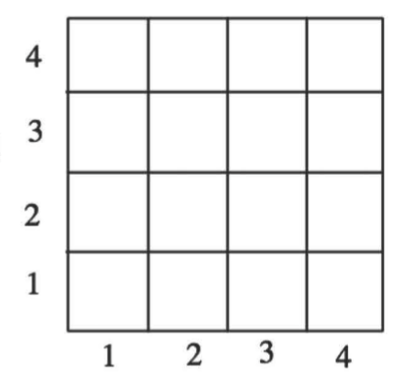
\includegraphics[width=0.45\textwidth]{L6_tworolls.png}
\eci 
}
{
\bci
\item<3-> \empr {Continuous case:} Dropping a needle in a plain

\bigskip
- $\Omega = \{(x,y) \in \real^2 \mid 0 \le x,y \le 1 \}$

\bigskip
\centering
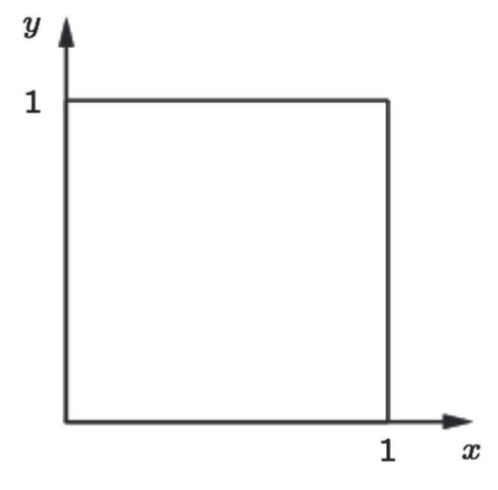
\includegraphics[width=0.5\textwidth]{L6_needle.png}
\eci 
}

\end{frame}

%%%%%%%%%%%%%%%%%%%%%%%%%%%%%%%%%%%%%%%%%%%%%%%%%%%%%%
\begin{frame}{Probability Law}

\plitemsep 0.1in

\bci

\item Assign numbers to what? Each outcome?

\item What is the probability of dropping a needle at $(0.5, 0.5)$ over the $1\times 1$ plane? 

\item Assign numbers to each \redf{subset} of $\Omega$: A subset of $\Omega$: \redf{an event}

\item $\cprob{A}$: Probability of an event $A.$

\bci
\item This is where probability meets set theory.  

\item Roll a dice. What is the probability of odd numbers?

\medskip
$
\cprob{ \{1,3,5 \}},
$
where $\{1,3,5 \} \subset \Omega$ is an event.
\eci

\item \redf{Event space \set{A}}: The collection of subsets of $\Omega.$ 
For example, in the discrete case, the power set of $\Omega.$ 

\item \redf{Probability Space $(\Omega,\set{A},\cprob{\cdot})$}
\eci

\end{frame}

%%%%%%%%%%%%%%%%%%%%%%%%%%%%%%%%%%%%%%%%%%%%%%%%%%%%%%
\begin{frame}{Random Variable: Idea}


\myvartwocols{0.7}{0.4}{0.57}
{
\plitemsep 0.1in

\bci 
\item In reality, many outcomes are \redf{numerical}, e.g., stock price.

\item Even if not, very convenient if we map numerical values to random outcomes, e.g., `0' for male and `1' for female.

\eci 
}
{
\centering
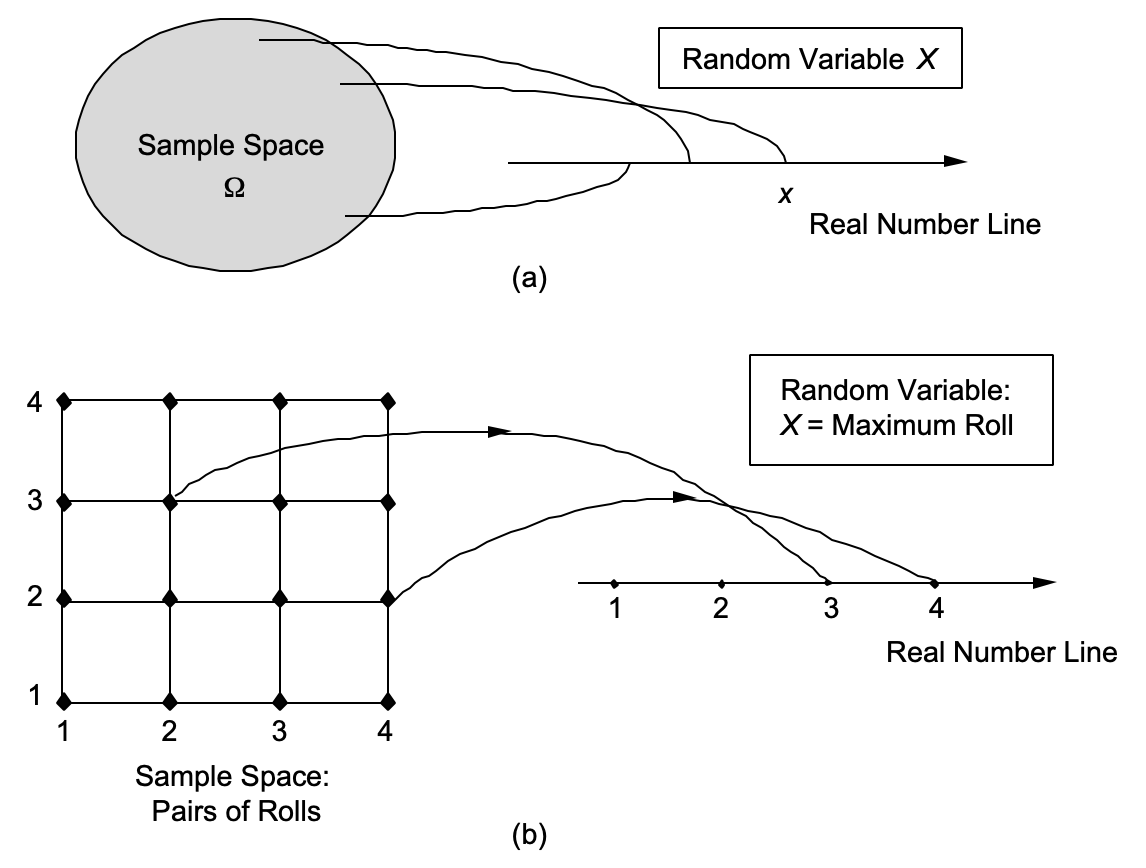
\includegraphics[width=0.9\textwidth]{L6_RV_ex.png}
}

\end{frame}

%%%%%%%%%%%%%%%%%%%%%%%%%%%%%%%%%%%%%%%%%%%%%%%%%%%%%%
\begin{frame}{Random Variable: More Formally}

\plitemsep 0.1in

\bci
\item Mathematically, a random variable $X$ is a \redblank{3}{function} which maps from $\Omega$ to $\real.$

\item \bluef{Notation.} Random variable $X$, numerical value $x.$

\item Different random variables $X$, $Y,$, etc can be defined on the same sample space. 

\item For a fixed value $x,$ we can associate an \redf{event} that a random variable $X$ has the value $x,$ i.e., 
\redf{$\{ \omega \in \Omega \mid X(w) = x \}$}

% \item Assume that values $x$ are discrete\footnote{Finite or countably infinite.} such as $1, 2, 3, \ldots.$

% For notational convenience,  
% $$
% \cprob{X = x} \ \eqdef \ \cbprob{\{ \omega \in \Omega \mid X(w) = x \}} 
% $$

\item Generally,
$$
\cprobi{X}{S} = \cprob{X \in S} = \cprob{\inv{X}(S)} = \cbprob{\{ \omega \in \Omega : X(w) \in S \}}
$$


\eci 

\end{frame}

%%%%%%%%%%%%%%%%%%%%%%%%%%%%%%%%%%%%%%%%%%%%%%%%%%%%%%
\begin{frame}{Conditioning: Motivating Example}

\plitemsep 0.1in
\bci 

\item Pick a person $a$ at random

- event $A$: $a$'s age $\leq$ 20

- event $B$: $a$ is married


\item (Q1) What is the probability of $A$?

\item (Q2) What is the probability of $A$, given that $B$ is true?

\item Clearly the above two should be different. 

\medskip

\item \question  How should I change my belief, given some additional information?

\item Need to build up a new theory, which we call \redf{conditional probability}.

\eci 

\end{frame}

%%%%%%%%%%%%%%%%%%%%%%%%%%%%%%%%%%%%%%%%%%%%%%%%%%%%%%
\begin{frame}{Conditional Probability}

%\plitemsep 0.1in
\bci

\item $\cprob{A \mid  B}$: $\cprob{\cdot | B}$ should be a new \redf{probability law.}

\item \defi
$$
\cprob{A \mid B} \eqdef \frac{\cprob{A \cap B}}{\cprob{B}}, \quad for \quad \cprob{B} >0.
$$

- Note that this is a \bluef{definition,} not a \bluef{theorem.}


\item All other properties of the law $\cprob{\cdot}$ is applied to the conditional law $\cprob{\cdot | B}.$ 

\item For example, for two disjoint events $A$ and $C$, 
$$
\cprob{A \cup C \redf{\ \mid B}} = \cprob{A \redf{\ \mid B}} + \cprob{C \redf{\ \mid B}}
$$

\eci 

\end{frame}

%%%%%%%%%%%%%%%%%%%%%%%%%%%%%%%%%%%%%%%%%%%%%%%%%%%%%%
\section{L6(2)}
\begin{frame}{Roadmap}

\plitemsep 0.1in

\bce[(1)]

\item \grayf{Construction of a Probability Space}
\item \redf{Discrete and Continuous Probabilities 
\item Sum Rule, Product Rule, and Bayes’ Theorem} 
\item \grayf{Summary Statistics and Independence
\item Gaussian Distribution
\item Conjugacy and the Exponential Family 
\item Change of Variables/Inverse Transform }

\ece
\end{frame}


%%%%%%%%%%%%%%%%%%%%%%%%%%%%%%%%%%%%%%%%%%%%%%%%%%%%%%
\begin{frame}{Discrete Random Variables}

\plitemsep 0.25in
\bci

\item The values that a random variable $X$ takes is discrete (i.e., finite or countably infinite). 

\item Then, $\px \eqdef \cprob{X = x} \eqdef \cbprob{\{ \omega \in \Omega \mid X(w) = x \}},$ which we call \redf{probability mass function} (PMF).

\item Examples: Bernoulli, Uniform, Binomial, Poisson, Geometric


\eci 

\end{frame}

%%%%%%%%%%%%%%%%%%%%%%%%%%%%%%%%%%%%%%%%%%%%%%%%%%%%%%
\begin{frame}{Bernoulli $X$ with parameter $p \in [0,1]$}

\plitemsep 0.1in

\bci
\item<1-> Only \redf{binary} values
\onslide<2->{
$$
X = \begin{cases}
0, & \text{w.p.\footnotemark} \quad 1-p, \cr
1, & \text{w.p.} \quad p
\end{cases}
$$
In other words, $p_X(0)=1-p$ and $p_X(1)=p$ from our PMF notation. }
\footnotetext{with probability}

\item<3-> Models a trial that results in binary results, e.g., success/failure, head/tail

\item<4-> Very useful for an \redblank{5}{indicator rv} of an event $A.$ 
\onslide<5->{
Define a rv $\indi{A}$ as:
$$
\indi{A} = 
\begin{cases}
1, & \text{if $A$ occurs}, \cr
0, & \text{otherwise}
\end{cases}
$$
}
\eci 

\end{frame}

%%%%%%%%%%%%%%%%%%%%%%%%%%%%%%%%%%%%%%%%%%%%%%%%%%%%%%
\begin{frame}{Uniform $X$ with parameter $a,b$}

\plitemsep 0.1in

\bci 
\item integers $a,b$, where $a \le b$

\item<2-> Choose a number of $\Omega = \{ a, a+1, \ldots, b \}$ uniformly at random. 

\item<3-> $p_X(i) = \frac{1}{b-a+1},$ $i \in \Omega.$

%\item $X(\omega) = \omega$

\centering
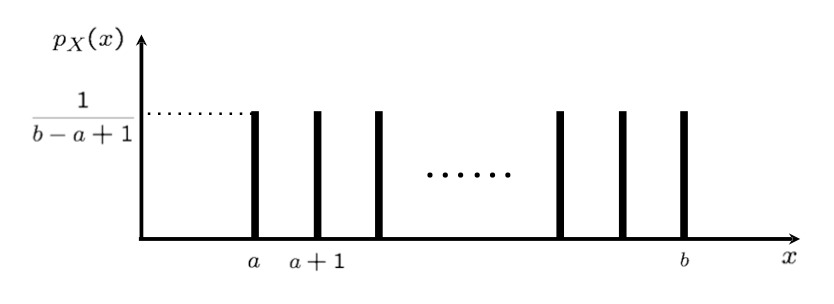
\includegraphics[width=0.7\textwidth]{L6_uniform_ex.png}

\item<4-> Models complete ignorance (I don't know anything about $X$)

\eci 

\end{frame}

%%%%%%%%%%%%%%%%%%%%%%%%%%%%%%%%%%%%%%%%%%%%%%%%%%%%%%
\begin{frame}{Binomial $X$ with parameter $n,p$}

\mytwocols{0.5}
{
\plitemsep 0.1in
\bci 
\item<2-> Models the number of successes in a given number of independent trials
\item<3-> $n$ independent trials, where one trial has the success probability $p.$

$$
p_X(k) = {n \choose k} p^k (1-p)^{n-k}
$$
\eci 
}
{
\centering
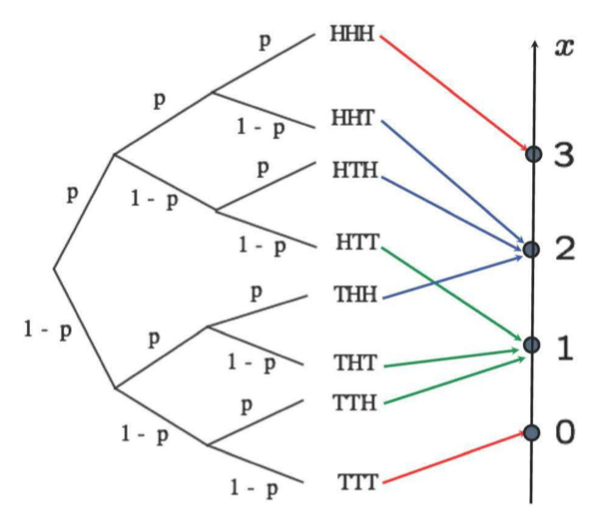
\includegraphics[width=0.8\textwidth]{L6_binomial_ex.png}
}
\end{frame}

%%%%%%%%%%%%%%%%%%%%%%%%%%%%%%%%%%%%%%%%%%%%%%%%%%%%%%
\begin{frame}{Poisson $X$ with parameter $\lambda$}

%\setdefaultleftmargin{0.1em}{}{}{}{}{}.

\plitemsep 0.05in
\bci 
\item<2-> $Binomial(n,p)$: Models the number of successes in a given number of independent trials with success probability $p.$

\item<3-> Very large $n$ and very small $p,$ such that $np =\lambda$
$$
p_X(k) = e^{-\lambda}\frac{\lambda^k}{k!}, \quad k=0,1, \ldots
$$

\item<4-> Is this a legitimate PMF?
\aleq{
\sum_{k=0}^\infty e^{-\lambda}\frac{\lambda^k}{k!} = e^{-\lambda} \left(1+ \lambda + \frac{\lambda^2}{2!} + \frac{\lambda^3}{3!} \ldots \right) = e^{-\lambda} e^\lambda = 1
}

\item<5-> Prove this:
$$
\lim_{n \rightarrow \infty} p_X(k) = {n \choose k} (1/n)^k (1-1/n)^{n-k} = e^{-\lambda}\frac{\lambda^k}{k!}
$$


\eci 

\end{frame}

%%%%%%%%%%%%%%%%%%%%%%%%%%%%%%%%%%%%%%%%%%%%%%%%%%%%%%
\begin{frame}{Geometric $X$ with parameter $p$}

\mytwocols{0.5}
{
\plitemsep 0.1in
\bci 
\item<1-> Experiment: infinitely many independent Bernoulli trials, where each trial has success probability $p$

\item<2-> Random variable: number of trials until the \redf{first success.} 

\item<3-> Models waiting times until something happens. 
$$
p_X(k) =  (1-p)^{k-1} p
$$
\eci 
}
{
\centering
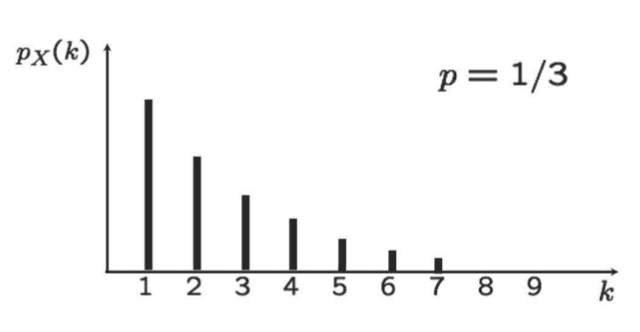
\includegraphics[width=0.8\textwidth]{L6_geo_ex.png}
}
\end{frame}

%%%%%%%%%%%%%%%%%%%%%%%%%%%%%%%%%%%%%%%%%%%%%%%%%%%%%%
\begin{frame}{Joint PMF}

\mytwocols{0.75}
{
\plitemsep 0.1in
\bci 

\item<2-> \redblank{3}{Joint PMF.} For two random variables $X,Y,$ consider two events
$\{X = x \}$ and $\{Y = y \},$ and
\aleq{
\onslide<3->{\redf{\pxy} \ \eqdef} \ \cbprob{\{X = x \} \cap \{Y = y \}}
}
\item<4-> $\sum_x \sum_y \pxy = 1$

\item<5-> \redblank{6}{Marginal PMF.} 
\aleq{
    \px &= \sum_{y} \pxy, \cr
    \py &= \sum_{x} \pxy
}

\eci 
}
{
Example.

\medskip
\centering
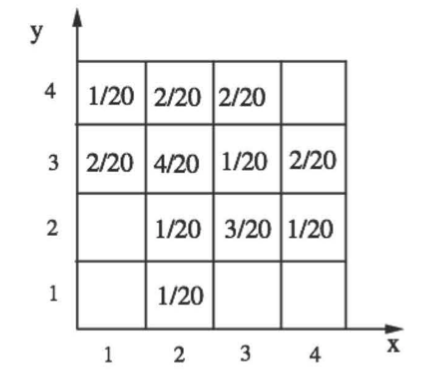
\includegraphics[width=0.5\textwidth]{L6_joint_ex.png}
\aleq{
p_{X,Y}(1,3)= 2/20
}
\aleq{
p_{X}(4) = 2/20 + 1/20 = 3/20
}
\aleq{
\cprob{X=Y}= 1/20 + 4/20 + 3/20 = 8/20
}
}
\end{frame}

%%%%%%%%%%%%%%%%%%%%%%%%%%%%%%%%%%%%%%%%%%%%%%%%%%%%%%
\begin{frame}{Conditional PMF}


\mytwocols{0.7}
{
\plitemsep 0.1in
\small

\bci 
\item \redf{Conditional PMF} 
\onslide<2->{
$$\pxcy \ \eqdef \ \cprob{X=x |{Y = y }} = \frac{\pxy}{\py}$$ 
for $y$ such that $\py >0.$}

\item<3-> $\sum_{x} \pxcy = 1$

\item \redf{Multiplication rule.}
\aleq{
\pxy &= \onslide<4->{\py \pxcy\cr    
     &= \px \pycx} 
}


\item $p_{X,Y,Z}(x,y,z) = \onslide<5->{\px \pycx p_{Z|X,Y}(z | x,y)}$
\eci 
}
{
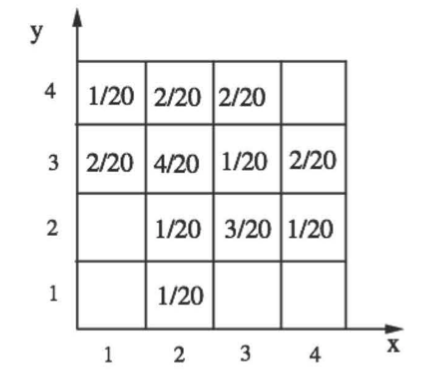
\includegraphics[width=0.5\textwidth]{L6_joint_ex.png}

\medskip
\small

$p_{X|Y}(2|2) = \frac{1}{1+3+1}$

\bigskip
$p_{X|Y}(3|2)= \frac{3}{1+3+1}$

\bigskip

$\expect{X | Y = 3} = 1(2/9)+ 2(4/9)+3(1/9)+4(2/9) $

}
\end{frame}

%%%%%%%%%%%%%%%%%%%%%%%%%%%%%%%%%%%%%%%%%%%%%%%%%%%%%%
\begin{frame}{Continuous RV and Probability Density Function (PDF)}
\small

\smallskip

\onslide<2->{- Many cases when random variable have ``continuous values", e.g., velocity of a car}
\onslide<3->{
\myblock{Continuous Random Variable}
{
A rv $X$ is \redf{continuous} if $\exists$ a function $f_X,$ called \redblk{probability density function (PDF)}, s.t. 
\vspace{-0.3cm}
$$
\cprob{X \in B} = \int_B \fx dx
$$
\vspace{-0.5cm}
}}
\vspace{-0.5cm}
\onslide<4->{- All of the concepts and methods (expectation, PMFs, and conditioning) for discrete rvs have continuous counterparts}
\vspace{-0.2cm}
\mytwocols{0.4}
{
\onslide<5->{
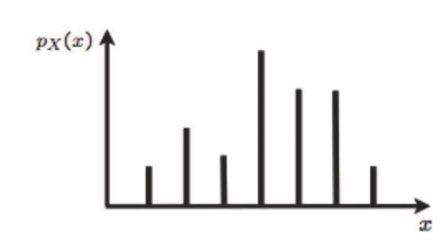
\includegraphics[width=0.65\textwidth]{L6_pmf_ex.png}
\vspace{-0.2cm}
\plitemsep 0.01in
\bci 
\item $\cprob{a \le X \le b} = \sum_{x: a\le x \le b} \px$
\item $\px \ge 0,$ $\sum_{x} \px = 1$
\eci} 
}
{
\onslide<6->{
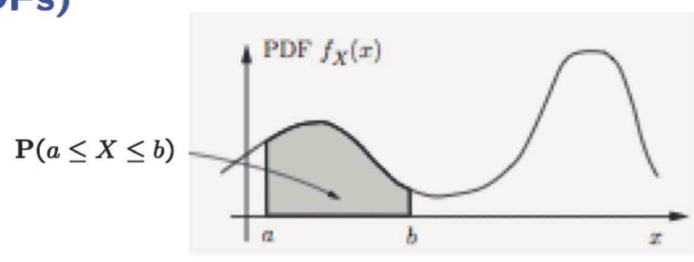
\includegraphics[width=0.85\textwidth]{L6_pdf_ex.png}

\plitemsep 0.01in
\bci 
\item $\cprob{a \le X \le b} = \int_{a}^b \fx dx$

\item $\fx \ge 0,$ $\int_{-\infty}^{\infty} \fx dx= 1$
\eci
} 
}
\end{frame}

%%%%%%%%%%%%%%%%%%%%%%%%%%%%%%%%%%%%%%%%%%%%%%%%%%%%%%
\begin{frame}{PDF and Examples}


\mytwocols{0.7}
{
\onslide<1->{
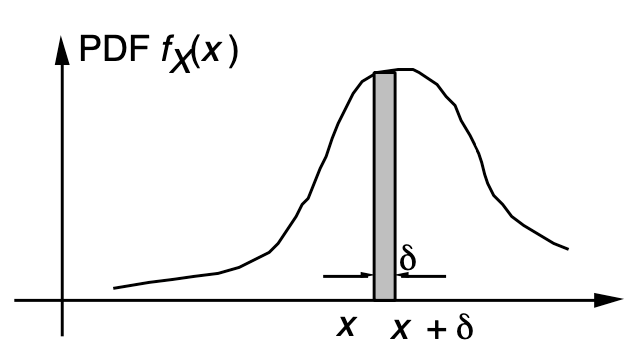
\includegraphics[width=0.65\textwidth]{L6_pdf_delta.png}

\bigskip

\plitemsep 0.1in
\bci 
\item $\cprob{a \le X \le a + \delta} \approx$ \redblank{2}{$f_X(a) \cdot \delta$}

\item \onslide<3->{$\cprob{X = a} = 0$}
\eci 
}
}
{
Examples

\onslide<4->{
\bigskip

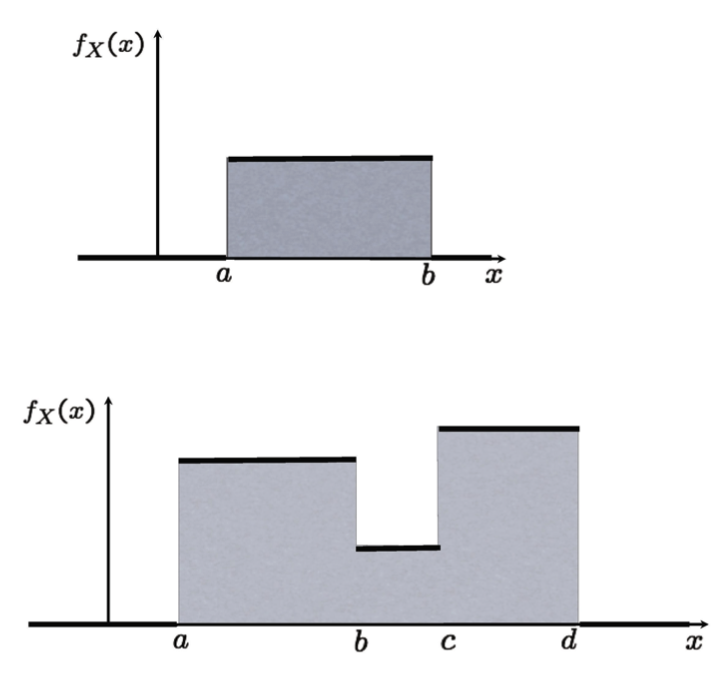
\includegraphics[width=0.8\textwidth]{L6_pdf_uniform_ex.png}
}
}
\end{frame}

%%%%%%%%%%%%%%%%%%%%%%%%%%%%%%%%%%%%%%%%%%%%%%%%%%%%%%
\begin{frame}{Cumulative Distribution Function (CDF)}

\mytwocols{0.8}
{
\small
\vspace{0.1in}
\plitemsep 0.1in
\bci 
\item<1-> Discrete: PMF, Continuous: PDF
\item<2-> Can we describe all rvs with a single mathematical concept? 
\onslide<3->{\aleq{
\Fx &= \cprob{X \le x} = \cr
& \begin{cases}
\sum_{k \le x} p_X(k), & \text{discrete}\cr
\int_{-\infty}^x f_X(t) dt, & \text{continuous}
\end{cases}
}}
\item<4-> always well defined, because we can always compute the probability for the event $\{X \le x \}$

\item<5-> CCDF (Complementary CDF): $\cprob{X > x }$
\eci 
}
{
\onslide<6->{\includegraphics[width=0.8\textwidth]{L6_cdf_ex1.png}}

\onslide<7->{\includegraphics[width=0.8\textwidth]{L6_cdf_ex2.png}}
}
\end{frame}

%%%%%%%%%%%%%%%%%%%%%%%%%%%%%%%%%%%%%%%%%%%%%%%%%%%%%%
\begin{frame}{CDF Properties}


\bigskip

\plitemsep 0.3in
\bci 
\item<2-> Non-decreasing

\item<3-> $F_X(x)$ tends to 1, as $x \rightarrow \infty$

\item<3-> $F_X(x)$ tends to 0, as $x \rightarrow -\infty$

\eci 
\bigskip

\end{frame}

%%%%%%%%%%%%%%%%%%%%%%%%%%%%%%%%%%%%%%%%%%%%%%%%%%%%%%
\begin{frame}{Exponential RV with parameter $\lambda >0$: $\exp(\lambda)$}

\plitemsep 0.02in
\bci 
\item<2-> A rv $X$ is called \redf{exponential with $\lambda$,} if
\aleq{
\fx = 
 \begin{cases}
 \lambda \elambdax, & x \ge 0 \cr
 0, & x <0
 \end{cases}
&\quad \text{or} \quad
\Fx = 1- \elambdax
}
\item<3-> Models a waiting time
\item<4-> CCDF $\cprob{X \ge x} = \elambdax$ (waiting time decays exponentially)
\item<5-> $\expect{X} = 1/\lambda$, $\expect{X^2} = 2/\lambda^2$, $\var{X} = 1/\lambda^2$
\item<6-> \redf{(Q)} What is the discrete rv which models a waiting time?  
\eci 

\vspace{-0.5cm}
\raggedleft
\onslide<2->{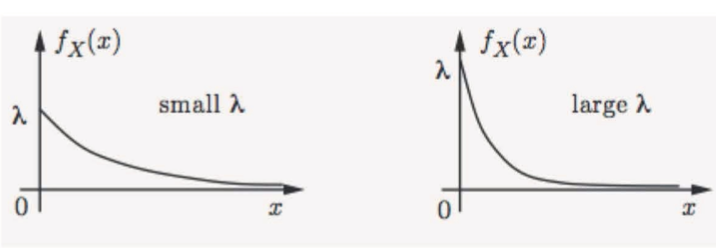
\includegraphics[width=0.5\textwidth]{L6_exp_pdf.png}}
%\mypic{0.9}{L4_exp_pdf.png}

\end{frame}
%%%%%%%%%%%%%%%%%%%%%%%%%%%%%%%%%%%%%%%%%%%%%%%%%%%%%%
\begin{frame}{Continuous: Joint PDF and CDF (1)}

\myblock{Jointly Continuous }
{
Two continuous rvs are \redblank{2}{jointly continuous} if a non-negative function $\fxy$ (called joint PDF) satisfies: for \redblk{every} subset $B$ of the two dimensional plane,
\aleq{
\cprob{(X,Y) \in B} = \iint_{(x,y) \in B} \fxy dx dy
}
\vspace{-0.3cm}
}

\plitemsep 0.1in
\bce 
\item<3-> The joint PDF is used to calculate probabilities  
$$\cprob{(X,Y) \in B} = \iint_{(x,y) \in B} \fxy dx dy$$

Our particular interest: $B = \{(x,y) \mid a \le x \le b, c \le y \le d \}$
\ece

\end{frame}

%%%%%%%%%%%%%%%%%%%%%%%%%%%%%%%%%%%%%%%%%%%%%%%%%%%%%%
\begin{frame}{Continuous: Joint PDF and CDF (2)}

\plitemsep 0.1in
\bce
\item<2->[2.] The marginal PDFs of $X$ and $Y$ are from the joint PDF as: 
$$
\fx = \int_{-\infty}^\infty \fxy dy, \quad \fy = \int_{-\infty}^\infty \fxy dx
$$

\item<3->[3.] The joint CDF is defined by $\Fxy = \cprob{X \le x, Y \le y},$ and determines the joint PDF as:
$$
\fxy = \frac{\partial^2 F_{x,y}}{\partial x \partial y} (x,y)
$$

\item<4->[4.] A function $g(X,Y)$ of $X$ and $Y$ defines a new random variable, and
$$
\expect{g(X,Y)} = \int_{-\infty}^\infty \int_{-\infty}^\infty g(x,y) \fxy dx dy
$$
\ece

\end{frame}

%%%%%%%%%%%%%%%%%%%%%%%%%%%%%%%%%%%%%%%%%%%%%%%%%%%%%%
\begin{frame}{Continuous:  Conditional PDF given a RV}

\plitemsep 0.2in
\bci 

\item $\pxcy = \frac{\pxy}{\py}$

\item<2-> Similarly, for $\fy >0,$
$$
\fxcy = \frac{\fxy}{\fy}
$$

\item<3-> Remember: For a fixed event $A,$ $\cprob{\cdot | A}$ is a legitimate probability law.

\item<4-> Similarly, For a fixed $y,$ $\fxcy$ is a legitimate PDF, since
$$
\int_{-\infty}^\infty \fxcy \redf{dx} = \frac{\int_{-\infty}^\infty \fxy dx}{\fy} = 1
$$
\eci
\end{frame}

% %%%%%%%%%%%%%%%%%%%%%%%%%%%%%%%%%%%%%%%%%%%%%%%%%%%%%%
% \begin{frame}{Continuous:  Conditional PDF given a RV}

% \mytwocols{0.8}
% {
% \medskip
% \small
% \plitemsep 0.1in
% \bci 

% \item $\pxcy = \frac{\pxy}{\py}$

% \item<2-> Similarly, for $\fy >0,$
% $$
% \fxcy = \frac{\fxy}{\fy}
% $$

% \item<3-> Remember: For a fixed event $A,$ $\cprob{\cdot | A}$ is a legitimate probability law.

% \item<4-> Similarly, For a fixed $y,$ $\fxcy$ is a legitimate PDF, since
% $$
% \int_{-\infty}^\infty \fxcy \redf{dx} = \frac{\int_{-\infty}^\infty \fxy dx}{\fy} = 1
% $$
% \eci
% }
% {
% \medskip
% \small
% \plitemsep 0.01in
% \bci 

% \item<5-> \redf{Multiplication rule.}
% \aleq{
% \fxy &= \fy \cdot \fxcy \cr
% &= \fx \fycx
% }

% \item<6-> \redf{Total prob./exp. theorem.}
% \aleq{
% \fx &= \int_{-\infty}^\infty \fy \fxcy dy \cr
% \expect{X | Y=y} &= \int_{-\infty}^\infty x \fxcy dx \cr
% \expect{X} &= \int_{-\infty}^\infty \fy \expect{X | Y=y} dy
% }

% \item<7-> \redf{Independence.}
% $$
% \fxy = \fx \fy, \quad \text{for all $x$ and $y$}
% $$
% \eci
% }
% \end{frame}

%%%%%%%%%%%%%%%%%%%%%%%%%%%%%%%%%%%%%%%%%%%%%%%%%%%%%%
\section{L6(3)}
\begin{frame}{Sum Rule and Product Rule}

\plitemsep 0.1in
\bci
\item \bluef{Sum Rule}
\aleq{
\px = \begin{cases}
\sum_{y \in \set{Y}} \pxy & \text{if discrete} \cr
\int_{y \in \set{Y}} \fxy dy & \text{if continuous}
\end{cases}
}

\bci
\item Generally, for $X = (X_1, X_2, \ldots, X_D),$
$$p_{X_i}(x_i) = \int p_{X}(x_1, \ldots, x_i, \ldots, x_D) d\vx_{-i}$$  
\item Computationally challenging, because of high-dimensional sums or integrals
\eci

\item \bluef{Product Rule}
\aleq{
\pxy &=  \px \cdot \pycx \cr
\text{\redf{joint} dist.} &= \text{\redf{marginal} of the first $\times$ \redf{conditional} dist. of the second given the first}
}
\vspace{-0.6cm}
\bci
\item Same as $\py \cdot \pxcy$
\eci

\eci
\end{frame}

% %%%%%%%%%%%%%%%%%%%%%%%%%%%%%%%%%%%%%%%%%%%%%%%%%%%%%%
% \begin{frame}{Bayesian Inference}

% \mytwocols{0.5}
% {
% \plitemsep 0.1in
% \bci 

% \item<2-> $A_1$: you are happy, $A_2$: you are sad
% \item<2-> $B$: you shout. 

% \item<4-> Assume that somebody gives you the following information:
% $$
% \cprob{A_1}, \quad \cprob{A_2}, \quad \cprob{B | A_1}, \quad\cprob{B | A_2}.
% $$

% \item<6-> \redf{Question:} $\cprob{A_1 | B}$ and $\cprob{A_2 | B}$?
% \eci 
% }
% {
% \plitemsep 0.1in
% \bci 

% \item<3-> $A_i$: state/cause/original value
% \item<3-> $B$: result/resulting action/noisy measurement

% \item<5-> In reality, $\cprob{A_i}$ (prior) and $\cprob{B | A_i}$ (cause $\rightarrow$ result) can be given from my model

% \item<7-> Inference: $\cprob{\text{cause} \mid \text{result}}$?

% \eci 
% }

% \end{frame}

% %%%%%%%%%%%%%%%%%%%%%%%%%%%%%%%%%%%%%%%%%%%%%%%%%%%%%%
% \begin{frame}{Total Probability Theorem}

% \mytwocols{0.7}
% {
% \plitemsep 0.1in
% \bci 

% \item<2-> Partition of $\Omega$ into $A_1,A_2,A_3$

% \item<3-> We know from my model: $\cprob{A_i}$ and $\cprob{B | A_i}$ 

% \item<4-> \redf{What is $\cprob{B}$? (probability of result)}

% %\bigskip

% \begin{block}<5->{Total Probability Theorem}
% $$
% \cprob{B} = \sum_{i} \cprob{A_i} \cprob{B | A_i}
% $$
% \end{block}

% \item<5-> $\cprob{A_i \cap B} = \cprob{A_i} \cprob{B | A_i}$

% \item<6-> Weighted average from the point of $A_i$ knowledge. 
% \eci 
% }
% {
% \centering
% \includegraphics[width=0.65\textwidth]{L2_total_ex.png}
% }

% \end{frame}

% %%%%%%%%%%%%%%%%%%%%%%%%%%%%%%%%%%%%%%%%%%%%%%%%%%%%%%
% \begin{frame}{Bayes' Rule}

% \mytwocols{0.7}
% {
% \plitemsep 0.1in

% \bci
% \item Partition of $\Omega$ into $A_1,A_2,A_3$

% \item We know from my model: $\cprob{A_i}$ and $\cprob{B | A_i}$ 

% \item<2-> \redf{What is $\cprob{A_i | B}$?}

% \item<2-> revised belief about $A_i,$ given $B$ occurs

% \begin{block}<3->{Bayes' Rule}
% $$
% \cprob{A_i | B} = \frac{\cprob{A_i} \cprob{B | A_i}}{\sum_{j} \cprob{A_j} \cprob{B | A_j}}
% $$
% \end{block}

% %\item Weighted average from the point of $A_i$ knowledge. 
% \eci 
% }
% {
% \centering
% \includegraphics[width=0.65\textwidth]{L2_total_ex.png}
% }

% \end{frame}

% %%%%%%%%%%%%%%%%%%%%%%%%%%%%%%%%%%%%%%%%%%%%%%%%%%%%%%
% \begin{frame}{Bayes' Rule: Example}

% \mytwocols{0.7}
% {
% \plitemsep 0.1in
% \bci 

% \item $A_1$: you are happy, $A_2$: you are sad
% \item $B$: you shout. 

% \item Assume: 
% $$
% \cprob{A_1}=0.7, \ \cprob{A_2}=0.3,
% $$
% $$
% \cprob{B | A_1} = 0.3, \ \cprob{B | A_2}=0.5.
% $$

% \eci 
% }
% {
% \medskip

% - Calculate $\cprob{A_1 | B}$ and $\cprob{A_2 | B}.$
% \aleq{
% \cprob{A_1} \cprob{B | A_1} &=  0.7 \times 0.3 = 0.21\cr
% \cprob{A_2} \cprob{B | A_2} &= 0.3 \times 0.5 = 0.15 \cr
% \cprob{B} &= 0.21 + 0.15 = 0.36
% }
% \aleq{
% \cprob{A_1 | B} = \frac{0.21}{0.36} \approx 0.583 \cr
% \cprob{A_2 | B} = \frac{0.15}{0.36} \approx 0.417 
% }
% }
% \end{frame}

%%%%%%%%%%%%%%%%%%%%%%%%%%%%%%%%%%%%%%%%%%%%%%%%%%%%%%
\begin{frame}{Bayes Rule}

\plitemsep 0.04in
\bci 

\item<1-> $X$: state/cause/original value $\rightarrow$ $Y$: result/resulting action/noisy measurement

\item<1-> Model: $\cprob{X}$ (prior) and $\cprob{Y | X}$ (cause $\rightarrow$ result)

\item<1-> Inference: $\cprob{X | Y}$?
 \mytwocols{0.35}
 {
\vspace{-0.2cm}
\onslide<2->{
\aleq{
\pxy & = \px \pycx \cr
     & = \py \pxcy \cr
\redf{\pxcy} & = \frac{\px \pycx}{\py}\cr
\py &= \sum_{x'} p_X(x')p_{Y|X}(y|x')
}
 }}
{
\vspace{-0.2cm}
\aleq{
\onslide<2->{
\fxy & = \fx \fycx \cr
     & = \fy \fxcy \cr
\redf{\fxcy} & = \frac{\fx \fycx}{\fy}\cr
\fy &= \int f_X(x')f_{Y|X}(y|x') dx'
}
}
}
\vspace{-0.4cm}
$$
\underbrace{\pxcy}_{\text{posterior}}  = \frac{\overbrace{\pycx}^{likelihood} \overbrace{\px}^{prior}}{\underbrace{\py}_{evidence}}
$$
\eci 
\end{frame}

%%%%%%%%%%%%%%%%%%%%%%%%%%%%%%%%%%%%%%%%%%%%%%%%%%%%%%
\begin{frame}{Bayes Rule for Mixed Case}

\onslide<1->{$K$: discrete, $Y$: continuous}

\bigskip

\plitemsep 0.1in
\mytwocols{0.5}
{
\bci 

\item<2-> Inference of $K$ given $Y$
\aleq{
\onslide<3->{
\redf{p_{K|Y}(k|y)} &= \frac{\redf{p_{K}(k)} \bluef{f_{Y|K}(y|k)}}{\bluef{\fy}}\cr
\bluef{\fy} &= \sum_{k'} \redf{p_{K}(k')} \bluef{f_{Y|K}(y|k')}
}}
\eci
}
{
\bci 

\item<2-> Inference of $Y$ given $K$
\aleq{
\onslide<4->{
\bluef{f_{Y|K}(y|k)} &= \frac{\bluef{\fy} \redf{p_{K|Y}(k|y)}}{\redf{p_{K}(k)}} \cr
\redf{p_{K}(k)} &= \int \bluef{f_{Y}(y')} \redf{p_{K|Y}(k|y')} dy'
}}
\eci 
}

\end{frame}



%%%%%%%%%%%%%%%%%%%%%%%%%%%%%%%%%%%%%%%%%%%%%%%%%%%%%%
\section{L6(4)}
\begin{frame}{Roadmap}

\plitemsep 0.1in

\bce[(1)] 

\item \grayf{Construction of a Probability Space}
\item \grayf{Discrete and Continuous Probabilities} 
\item \grayf{Sum Rule, Product Rule, and Bayes’ Theorem} 
\item \redf{Summary Statistics and Independence}
\item \grayf{Gaussian Distribution
\item Conjugacy and the Exponential Family 
\item Change of Variables/Inverse Transform }

\ece
\end{frame}

%%%%%%%%%%%%%%%%%%%%%%%%%%%%%%%%%%%%%%%%%%%%%%%%%%%%%%
\begin{frame}{Independence}

\plitemsep 0.05in
\bci 

\item<1-> Occurrence of $A$ provides no new information about $B.$ Thus, knowledge about $A$ does no change my belief about $B.$ 
\onslide<2->{
\bluef{
$$
\cprob{B | A} = \cprob{B}
$$
}}

\item Using $\cprob{B | A} = \cprob{B \cap A}/\cprob{A},$ 

\begin{block}<3->{Independence of $A$ and $B$, \redblank{4}{$A \indep B$}}
$\cprob{A \cap B} = \cprob{A} \times \cprob{B}$
\end{block}

\item<5-> \redf{Q1.} $A$ and $B$ disjoint $\imp$ $A \indep B$?

\onslide<6->{
No. Actually, really dependent, because if you know that $A$ occurred, then, we know that $B$ did not occur. 
}

\item<7-> \redf{Q2.} If $A \indep B$,  then $A \indep B^c$? \onslide<8->{Yes.} 
\eci 
\end{frame}

%%%%%%%%%%%%%%%%%%%%%%%%%%%%%%%%%%%%%%%%%%%%%%%%%%%%%%
\begin{frame}{Conditional Independence}

\plitemsep 0.07in
\bci 

\item<2-> Remember: for a probability law $\cprob{\cdot},$ given, say $B$, $\cprob{\cdot | B}$ is a new probability law. 

\item<3-> Thus, we can talk about independence under $\cprob{\cdot | B}.$

\item<4-> Given that $C$ occurs, occurrence of $A$ provides no new information about $B.$
$$
\cprob{B | A \cap C} = \cprob{B | C}
$$
\vspace{-0.2in}
%\item Using $\cprob{B | A} = \cprob{B \cap A}/\cprob{A},$ 
\begin{block}<5->{Conditional Independence of $A$ and $B$ given $C$, \redblank{6}{$A \indep B | C$}}
$\cprob{A \cap B | C} = \cprob{A |C} \times \cprob{B |C}$
\end{block}

\smallskip
\item<7-> \redf{Q1.} If $A \indep B$,  then $A \indep B | C$?
Suppose that $A$ and $B$ are independent. If you heard that $C$ occurred,  $A$ and $B$ are still independent?                                                         

\item<8-> \redf{Q2.} If $A \indep B | C$, $A \indep B$?
\eci 
\end{frame}

%%%%%%%%%%%%%%%%%%%%%%%%%%%%%%%%%%%%%%%%%%%%%%%%%%%%%%
\begin{frame}{$A \indep B$ $\rightarrow$  $A \indep B | C$?}

\plitemsep 0.2in
\bci 

\item<1-> Two independent coin tosses

\plitemsep 0.05in
\bci
\item $H_1$: 1st toss is a head
\item $H_2$: 2nd toss is a head
\item $D$: two tosses have different results.
\eci

\item<2-> $\cprob{H_1 | D} = 1/2,$ $\cprob{H_2 | D} = 1/2$  


\item<3-> $\cprob{H_1 \cap H_2 | D} = 0,$  

\item<3-> No.
\eci 
\end{frame}

%%%%%%%%%%%%%%%%%%%%%%%%%%%%%%%%%%%%%%%%%%%%%%%%%%%%%%
\begin{frame}{$A \indep B | C$ $\rightarrow$  $A \indep B$?}

\myvartwocols{0.8}{0.7}{0.27}
{
\small
\plitemsep 0.02in
\bci 

\item<1-> Two coins: \bluef{Blue} and \redf{Red}. Choose one uniformly at random, and proceed with two independent tosses. 

\item<2-> $\cprob{\text{head of blue}} = 0.9$ and 
$\cprob{\text{head of red}} = 0.1$ 

$H_i$: i-th toss is head, and $B$: blue is selected. 

\item<3-> $H_1 \indep H_2 | B$? Yes
\aleq{
\cprob{H_1 \cap H_2 | B} = 0.9\times 0.9, \quad \cprob{H_1 |B} \cprob{H_2|B} = 0.9 \times 0.9
}

\item<4-> $H_1 \indep H_2$? No
\abovedisplayskip=-0.01in
\aleq{
\onslide<5->{\cprob{H_1} &= \cprob{B} \cprob{H_1 | B} + \cprob{B^c} \cprob{H_1 | B^c} \cr
&= \frac{1}{2} 0.9 + \frac{1}{2} 0.1 = \frac{1}{2}\cr
\cprob{H_2} &= \cprob{H_2} \quad (\text{because of symmetry})\cr}
\onslide<6->{\cprob{H_1 \cap H_2} &= \cprob{B} \cprob{H_1 \cap H_2| B} + \cprob{B^c} \cprob{H_1 \cap H_2| B^c}\cr 
& = \frac{1}{2} (0.9\times 0.9) + \frac{1}{2} (0.1\times 0.1) \neq \frac{1}{2}}
}
\eci 
}
{
\centering
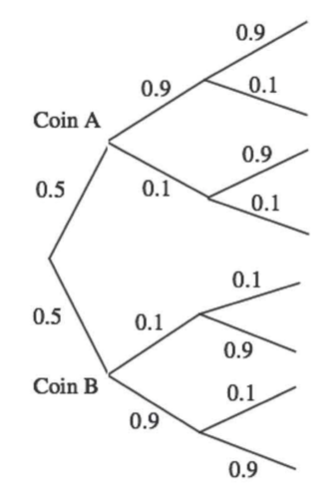
\includegraphics[width=0.8\textwidth]{L6_condind_ex.png}
}


\end{frame}

%%%%%%%%%%%%%%%%%%%%%%%%%%%%%%%%%%%%%%%%%%%%%%%%%%%%%%
\begin{frame}{Independence for Random Variables}

\bci 
\item<4-> Two rvs
\aleq{
\cprob{ \{X = x \} \cap \{Y=y \}} &= \cprob{X=x} \cdot \cprob{Y=y}, \quad \text{for all $x,y$}\cr
\onslide<5->{\pxy&= \px \cdot \py}
}
\aleq{
\cprob{ \{X = x \} \cap \{Y=y \}\redf{|C}} &= \cprob{X=x\redf{|C}} \cdot \cprob{Y=y\redf{| C}}, \quad \text{for all $x,y$}\cr
\onslide<5->{p_{X,Y\redf{|C}}(x,y)&=p_{X\redf{|C}}(x) \cdot p_{Y\redf{|C}}(y)}
}

\item Notation: $X \indep Y$ (independence), $X \indep Y | Z (conditional independence)$
\eci 


\end{frame}

%%%%%%%%%%%%%%%%%%%%%%%%%%%%%%%%%%%%%%%%%%%%%%%%%%%%%%
\begin{frame}{Expectation/Variance}

\mytwocols{0.7}
{
\plitemsep 0.1in
\bci
\item Expectation
\aleq{
\expect{X} = \sum_{x} x \px , \quad \expect{X} = \int_x x\fx dx
}

\item Variance, Standard deviation

\vspace{0.3cm}
- Measures how much the spread of PMF/PDF is

\aleq{
    \var{X} &= \expect{(X-\mu)^2} \cr
    \sigma_X &= \sqrt{\var{X}}
}
\eci
}
{
Properties

\medskip
\bci
\item $\expect{aX + bY +c} = a\expect{X} + b\expect{Y} + c$

\item $\var{aX +b} = a^2 \var{X}$

\item $\var{X + Y} = \var{X} + \var{Y}$ if $X \indep Y$ (generally not equal)
\eci
}

\end{frame}

%%%%%%%%%%%%%%%%%%%%%%%%%%%%%%%%%%%%%%%%%%%%%%%%%%%%%%
\begin{frame}{Covariance}

\plitemsep 0.1in

\bci 

\item<1-> Goal: Given two rvs $X$ and $Y$, quantify the degree of their dependence
\bci
\item<1-> Dependent: Positive (If $X \uparrow$, $Y \uparrow$) or Negative (If $X \uparrow,$ $Y \downarrow$)
\item<2-> Simple case: $\expect{X} =\mu_x = 0$ and $\expect{Y}=\mu_Y = 0$
\eci

\medskip
\mytwocols{0.4}
{
\bci
\item<3-> What about $\expect{XY}$? Seems good. 
\item<4-> $\expect{XY} = \expect{X}\expect{Y}=0$ when $X \indep Y$
\item<5-> More data points (thus increases) when $xy >0$ (both positive or negative)
\eci
}
{
\centering
\onslide<5->{\mypic{0.8}{L6_cov_ex.png}}
}

\eci

\end{frame}

%%%%%%%%%%%%%%%%%%%%%%%%%%%%%%%%%%%%%%%%%%%%%%%%%%%%%%
\begin{frame}{What If $\mu_X \neq 0, \mu_Y \neq 0$?}

\plitemsep 0.1in

\bci 

\item<2-> Solution: Centering. $X \rightarrow X - \mu_X$ and $Y \rightarrow Y-\mu_Y$
\onslide<3->{
\myblock{Covariance}
{
$\cov{X,Y} = \bexpect{(X- \expect{X})\cdot (Y-\expect{Y})}$
}}

\item<4-> After some algebra, $\cov{X,Y} = \expect{XY} - \expect{X}\expect{Y}$

\item<5-> $X \indep Y$ $\imp$ $\cov{X,Y}=0$

\item<6-> $\cov{X,Y}=0$ $\imp$ $X \indep Y$? NO.

\item<7-> When $\cov{X,Y}=0,$ we say that $X$ and $Y$ are \redblank{8}{uncorrelated.}

\eci

\end{frame}

%%%%%%%%%%%%%%%%%%%%%%%%%%%%%%%%%%%%%%%%%%%%%%%%%%%%%%
\begin{frame}{Example: $\cov{X,Y}=0,$ but not independent}

\plitemsep 0.1in

\bci 

\item $p_{X,Y}(1,0) = p_{X,Y}(0,1) = p_{X,Y}(-1,0) = p_{X,Y}(0,-1) = 1/4.$

\item<2-> $\expect{X} = \expect{Y}=0,$ and $\expect{XY}=0.$ So, $\cov{X,Y}=0$

\item<3-> Are they independent? No, because if $X=1$, then we should have $Y=0.$

\eci
\centering
\mypic{0.3}{L6_cov_notind.png}
\end{frame}

%%%%%%%%%%%%%%%%%%%%%%%%%%%%%%%%%%%%%%%%%%%%%%%%%%%%%%
\begin{frame}{Properties}

\plitemsep 0.07in

\vspace{-0.3in}
\bci []

\item<2-> \aleq{
\cov{X,X}=0
}

\item<3-> \aleq{
\cov{aX +b, Y} &= \expect{(aX+b)Y} - \expect{aX+b}\expect{Y} = a\cdot \cov{X,Y}
}

\item<4->  \aleq{
\cov{X,Y+Z} &= \expect{X(Y+Z)} - \expect{X}\expect{Y+Z}= \cov{X,Y} + \cov{X,Z}
}

\item<5-> \aleq{
\var{X+Y} &= \expect{(X+Y)^2} - (\expect{X+Y})^2 = \var{X} + \var{Y} - 2\cov{X,Y}
}
\eci

\end{frame}

%%%%%%%%%%%%%%%%%%%%%%%%%%%%%%%%%%%%%%%%%%%%%%%%%%%%%%
\begin{frame}{Correlation Coefficient: Bounded Dimensionless Metric}

\plitemsep 0.1in

\bci 

\item \redf{Always bounded by some numbers, e.g., $[-1,1]$}

\item<3-> Dimensionless metric. How? \redblank{4}{Normalization,} but by what?

\onslide<5->{
\myblock{Correlation Coefficient}
{
\aleq{
\rho(X,Y) = \bbexpect{\frac{(X - \mu_X)}{\redf{\sigma_X}} \cdot \frac{Y-\mu_Y}{\redf{\sigma_Y}}} = \frac{\cov{X,Y}}{\sqrt{\var{X}\var{Y}}}
}
}
}
\item<6-> $-1 \le \rho \le 1$

\item<7-> $|\rho|=1$ $\imp$ $X-\mu_X = c(Y-\mu_Y)$ (linear relation, VERY related)

\eci

\end{frame}
%%%%%%%%%%%%%%%%%%%%%%%%%%%%%%%%%%%%%%%%%%%%%%%%%%%%%%
\begin{frame}{}
\vspace{2cm}
\LARGE Extension to Random Vectors $\vec{X} = \colvec{X_1 \\ \vdots \\ X_n}$


\end{frame}

%%%%%%%%%%%%%%%%%%%%%%%%%%%%%%%%%%%%%%%%%%%%%%%%%%%%%%
\begin{frame}{Expectation, Covariance, Variance}

\plitemsep 0.1in

\bci 

\item $\cexpect{\vX} \eqdef \colvec{\cexpect{X_1} \\ \vdots \\ \cexpect{X_n}}$

\item Covariance of $\vX \in \realn$ and $\vY \in \realm$
$$
\cov{\vX,\vY} = \cexpect{\vX \trans{\vY}} - \cexpect{\vX} \trans{\cexpect{\vY}} \in \realnm
$$

\item Variance of $\vX$: $\cvar{\vX} = \cov{\vX,\vX} \in \realnn,$ often denoted by $\msig_{\vX}$ (or simply $\msig$):
$$
\msig_{\vX} \eqdef \var{\vX} = \begin{nmat}
\cov{X_1,X_1} & \cov{X_1,X_2} & \cdots \cov{X_1,X_n} \cr
\vdots & \vdots & \vdots \cr
\cov{X_n,X_1} & \cov{X_n,X_2} & \cdots \cov{X_n,X_n} \cr
\end{nmat}
$$
\bci
\item We call $\msig_{\vX}$ \bluef{covariance matrix} of $\vX.$
\eci

\eci
\end{frame}

%%%%%%%%%%%%%%%%%%%%%%%%%%%%%%%%%%%%%%%%%%%%%%%%%%%%%%
\begin{frame}{Data Matrix and Data Covariance Matrix }

\plitemsep 0.05in

\bci 
\item $N$: number of samples, $D$: number of measurements (or original features)
\item iid dataset $\cX = \{\vx_1, \ldots, \vx_N \}$ whose mean is $\vec{0}$ (well-centered), where each $\vx_i \in \realD,$ and its corresponding data matrix 
$$\mX = \rowvec{\vx_1 & \cdots & \vx_N} =\generalmatrix{x}{N}{D}
\in \real^{D \times N}$$

\item \bluef{(data) covariance matrix}  \hfill \lecturemark{L10(1)}
\mycolorbox{
$$\mS = \dfrac{1}{N} \mX\trans{\mX} = \dfrac{1}{N} \sum_{n=1}^N \vx_n \trans{\vx}_n \in \real^{D\times D}$$
}

\eci

\end{frame}

%%%%%%%%%%%%%%%%%%%%%%%%%%%%%%%%%%%%%%%%%%%%%%%%%%%%%%
\begin{frame}{Covariance Matrix and Data Covariance Matrix}

\plitemsep 0.1in

\bci
\item \question Relation between covariance matrix and data covariance matrix?
\item Covaiance matrix for a random vector $\vY = \trans{(Y_1, \ldots, Y_D)},$ 
$$
\msig_{\vY}  = \begin{nmat}
\cov{Y_1,Y_1} & \cov{Y_1,Y_2} & \cdots \cov{Y_1,Y_D} \cr
\vdots & \vdots & \vdots \cr
\cov{Y_D,Y_1} & \cov{Y_n,Y_2} & \cdots \cov{Y_D,Y_D} \cr
\end{nmat}
$$

\item Data convariance matrix $\mS \in \real^{D\times D}$

\bci
\item Each $Y_i$ has $N$ samples $\rowvec{x_{i,1} & \cdots & x_{i,N}}$
\eci
\begin{eqnarray*}
\mS_{ij}= \cov{Y_i, Y_j} &=& \frac{1}{N}\sum_{k=1}^N x_{i,k} \cdot x_{j,k} \cr
&=&\text{ average covariance (over samples) btwn feastures $i$ and $j$}
\end{eqnarray*}

\eci

\end{frame}


% %%%%%%%%%%%%%%%%%%%%%%%%%%%%%%%%%%%%%%%%%%%%%%%%%%%%%%
% \begin{frame}{\redf{Data} Covariance Matrix}

% {\Large \red 뒤에 나올 data covariance matrix를 여기서 한번 보여준다.}

% \plitemsep 0.1in

% \bci 

% \item 

% \eci
% \end{frame}

%%%%%%%%%%%%%%%%%%%%%%%%%%%%%%%%%%%%%%%%%%%%%%%%%%%%%%
\begin{frame}{Properties}

For two random vectors $\vX, \vY \in \realn,$

\plitemsep 0.1in

\bci 

\item $\cexpect{\vX + \vY} = \cexpect{\vX} + \cexpect{\vY} \in \realn$ 

\item $\cvar{\vX + \vY} = \cvar{\vX} + \cvar{\vY} \in \realnn$


\item Assume $\vY = \mA \vX + \vb.$
\bci
\item $\cexpect{\vY} = \mA \cexpect{\vX} + \vb$
\item $\cvar{\vY} = \cvar{\mA\vX} = \mA \: \cvar{\vX} \trans{\mA}$
\item $\cov{\vX,\vY} = \msig_{\vX}\trans{\mA}$ (Please prove)
\eci
\eci
\end{frame}


%%%%%%%%%%%%%%%%%%%%%%%%%%%%%%%%%%%%%%%%%%%%%%%%%%%%%%
\section{L6(5)}
\begin{frame}{Roadmap}

\plitemsep 0.1in

\bce[(1)] 

\item \grayf{Construction of a Probability Space}
\item \grayf{Discrete and Continuous Probabilities} 
\item \grayf{Sum Rule, Product Rule, and Bayes’ Theorem} 
\item \grayf{Summary Statistics and Independence}
\item \redf{Gaussian Distribution}
\item \grayf{Conjugacy and the Exponential Family 
\item Change of Variables/Inverse Transform }

\ece
\end{frame}

%%%%%%%%%%%%%%%%%%%%%%%%%%%%%%%%%%%%%%%%%%%%%%%%%%%%%%
\begin{frame}{Normal (also called Gaussian) Random Variable}


\plitemsep 0.1in
\bci 
\item Why important?
\bci
\item Central limit theorem (중심극한정리)

- One of the most remarkable findings in the probability theory

\item Convenient analytical properties

\item Modeling aggregate noise with many small, independent noise terms
\eci
\eci
\mysmalltwocols{0.4}
{
\plitemsep 0.1in
\bci 
\item<1-> Standard Normal $\set{N}(0,1)$
\aleq{
\fx & = \frac{1}{\sqrt{2\pi}} e^{-x^2/2}
}
\item<1-> $\expect{X} = 0$

\item<1-> $\var{X} = 1$
\eci
}
{
\plitemsep 0.1in
\bci 
\item<2-> General Normal $\set{N}(\mu, \sigma^2)$
\aleq{
\fx & = \frac{1}{\sigma\sqrt{2\pi}} e^{-(x-\mu)^2/2\sigma^2}
}

\item<2-> $\expect{X} = \mu$

\item<2-> $\var{X} = \sigma^2$

\eci
}

\end{frame}



%%%%%%%%%%%%%%%%%%%%%%%%%%%%%%%%%%%%%%%%%%%%%%%%%%%%%%
\begin{frame}{Gaussian Random Vector}

\plitemsep 0.1in
\bci 
\item $\vX = \trans{(X_1, X_2, \cdots, X_n)}$ with the mean vector $\vmu = \colvec{\cexpect{X_1} \\ \vdots \\ \cexpect{X_n}}$ and the covariance matrix $\msig.$

\item A Gaussian random vector $\vX = \trans{(X_1, X_2, \cdots, X_n)}$ has a joint pdf of the form:
$$
f_{\vX}(\vx) = \frac{1}{\sqrt{(2\pi)^n |\msig|}} \exp\left(-\frac{1}{2}\trans{(\vx - \vmu)} \inv{\msig}(\vx - \vmu) \right),
$$
where $\msig$ is symmetric and positive definite. 

\item We write $\vX \sim \set{N}(\vmu, \msig),$ or $p_{\vX}(\vx) = \set{N}(\vx \mid \vmu, \msig).$
\eci
\end{frame}

%%%%%%%%%%%%%%%%%%%%%%%%%%%%%%%%%%%%%%%%%%%%%%%%%%%%%%
\begin{frame}{Power of Gaussian Random Vectors}

\plitemsep 0.2in
\bci 
\item Marginals of Gaussians are Gaussians
\item Conditionals of Gaussians are Gaussians
\item Products of Gausssian Densities are Gaussians.
\item A sum of two Gassuaians is Gaussian if they are independent 
\item Any linear/affine transformation of a Gaussian is Gaussian. 
\eci
\end{frame}

%%%%%%%%%%%%%%%%%%%%%%%%%%%%%%%%%%%%%%%%%%%%%%%%%%%%%%
\begin{frame}{Marginals and Conditionals of Gaussians}

\plitemsep 0.03in
\bci 
\item $\vX$ and $\vY$ are Gaussians with mean vectors $\vmu_{\vX}$ and $\vmu_{\vY},$ respectively.
\item Gaussian random vector $\vZ = \colvec{\vX \\ \vY}$ with $\vmu = \colvec{\vmu_{\vX} \\ \vmu_{\vY}}$ and the covarance matrix $\msig_{\vZ} = 
\begin{nmat} 
\msig_{\vX} & \msig_{\vX\vY} \cr
\msig_{\vY\vX} & \msig_{\vY} 
\end{nmat},$  
where $\msig_{\vX\vY} = \cov{\vX,\vY}.$

\medskip
\mytwocols{0.4}
{
- \redf{Marginal.} 
\aleq{f_{\vX}(\vx)= \int f_{\vX,\vY}(\vx,\vy) d\vy \sim \set{N}(\vmu_{\vx}, \msig_{\vX})
}

\medskip
- \redf{Conditional.} $\vX \mid \vY \sim \set{N}(\vmu_{\vX | \vY}, \msig_{\vX | \vY}),$ 
% \medskip
% where 
\aleq{
\vmu_{\vX | \vY} & = \vmu_{\vX} + \msig_{\vX \vY}\inv{\msig_{\vY}}(\vY - \vmu_{\vY}) \cr
\msig_{\vX | \vY} &= \msig_{\vX} - \msig_{\vX \vY}\inv{\msig_{\vY}}\msig_{\vY \vX}
}
}
{
\vspace{-0.3cm}
\mypic{0.8}{L6_marginal_conditional.png}
}
\eci
\end{frame}

%%%%%%%%%%%%%%%%%%%%%%%%%%%%%%%%%%%%%%%%%%%%%%%%%%%%%%
\begin{frame}{Product of Two Gaussian Densities}

\plitemsep 0.1in
\bci 
\item \redf{Lemma.} Up to recaling, the pdf of the form $\exp(-\frac{1}{2} ax^2 -2bx +c)$ is $\set{N}(\frac{b}{a},\frac{1}{a}).$  

\medskip
\item Using the above Lemma, the product of two Gaussians $\set{N}(\mu_0,\nu_0)$ and $\set{N}(\mu_1,\nu_1)$ is Gaussian up to rescaling. 

\medskip
\bluef{Proof.}
\aleq{
&\exp \left(-(x-\mu_0)^2/2\nu_0 \right) \times \exp\left(-(x-\mu_1)^2/2\nu_1\right) \cr
&= \exp\left[-\frac{1}{2}\left(\Bl(\frac{1}{\nu_0} + \frac{1}{\nu_1}\Br)x^2 -2 \Bl(\frac{\mu_0}{\nu_0} + \frac{\mu_1}{\nu_1}\Br)x + c \right) \right ] \cr
& \implies \set{N}\left(\overbrace{\frac{1}{\inv{\nu_0} + \inv{\nu_1}}}^{= \nu} , \nu 
\left(\frac{\mu_0}{\nu_0} + \frac{\mu_1}{\nu_1}\right) \right)
= \set{N}\left(\frac{\nu_1\mu_0 + \nu_0\mu_1}{\nu_0 + \nu_1}, \frac{\nu_0\nu_1}{\nu_0+\nu_1} \right)
}

\eci
\end{frame}

%%%%%%%%%%%%%%%%%%%%%%%%%%%%%%%%%%%%%%%%%%%%%%%%%%%%%%
\begin{frame}{Product of Two Gaussian Densities for Random Vectors}

\plitemsep 0.1in
\bci 
\item Similar results for the matrix version.

\item The product of the densities of two Gaussian vectors $\set{N}(\vmu_0,\msig_0)$ and $\set{N}(\vmu_1,\msig_1)$ is Gaussian up to rescaling. 

\item The resulting Gaussian is given by:
$$
\set{N}\Bigg(\msig_1 \inv{(\msig_0 + \msig_1)} \vmu_0 + \msig_0\inv{(\msig_0 + \msig_1)}\vmu_1,
\msig_1\inv{(\msig_0 + \msig_1)}\msig_0
\Bigg)
$$
\bluef{Compare the above to this:}
$$
\set{N}\Bigg(\frac{\nu_1\mu_0 + \nu_0\mu_1}{\nu_0 + \nu_1}, \frac{\nu_0\nu_1}{\nu_0+\nu_1} \Bigg)
$$
\eci
\end{frame}

%%%%%%%%%%%%%%%%%%%%%%%%%%%%%%%%%%%%%%%%%%%%%%%%%%%%%%
\begin{frame}{Formula: Conditional and Marginal Gaussians}

\mypic{0.5}{L6_gaussian_formula.png}

\footnotetext{Source: Pattern Recognition and Machine Learning, Springer by Christopher M. Bishop}
\end{frame}

%%%%%%%%%%%%%%%%%%%%%%%%%%%%%%%%%%%%%%%%%%%%%%%%%%%%%%
\begin{frame}{Sum of Gaussians}

\plitemsep 0.5in
\bci 
\item $\vX \sim \set{N}(\vmu_{\vX}, \msig_{\vX})$ and $\vY \sim \set{N}(\vmu_{\vY}, \msig_{\vY})$

\item[$\implies$] $a\vX + b\vY \sim \set{N}(a\vmu_{\vX} + b\vmu_{\vY}, a^2\msig_{\vX} + b^2\msig_{\vY})$


\eci
\end{frame}

%%%%%%%%%%%%%%%%%%%%%%%%%%%%%%%%%%%%%%%%%%%%%%%%%%%%%%
\begin{frame}{Mixture of Two Gaussian Densities}

\plitemsep 0.1in
\bci 
\item $f_1(x)$ is the density of $\set{N}(\mu_1,\sigma_1^2)$ and $f_2(x)$ is the density of $\set{N}(\mu_2,\sigma_2^2)$

%$\vX \sim \set{N}(\vmu_{\vX}, \msig_{\vX})$ and $\vY \sim \set{N}(\vmu_{\vY}, \msig_{\vY})$

\item \question What are the mean and the variance of the random variable $Z$ which has the following density $f(x)$?
$$
f(x) = \alpha f_1(x) + (1-\alpha)f_2(x)
$$
\bluef{Answer:}

\aleq{
\cexpect{Z} &= \alpha \mu_1 + (1-\alpha)\mu_2\cr
\cvar{Z} &= \Big(\alpha \sigma_1^2 + (1-\alpha)\sigma_2^2 \Big) + \Big([\alpha \mu_1^2 + (1-\alpha)\mu_2^2] - [\alpha \mu_1 + (1-\alpha)\mu_2]^2 \Big)
}
\eci
\end{frame}

%%%%%%%%%%%%%%%%%%%%%%%%%%%%%%%%%%%%%%%%%%%%%%%%%%%%%%
\begin{frame}{Linear Transformation}

\plitemsep 0.1in
\bci 
\item<2-> Linear transformation\footnote{Strictly speaking, this is affine transformation.} preserves normality

\myblock{Linear transformation of Normal}
{
If $X \sim  \set{N}(\mu, \sigma^2) $, then for $a \neq 0$ and $b,$ $Y = aX +b \sim \set{N}(a\mu +b,a^2 \sigma^2).$ 
}

\item<3-> Thus, every normal rv can be \redblank{4}{standardized}: 

If $X \sim  \set{N}(\mu, \sigma^2)$, then 
\redblank{4}{$Y = \frac{X-\mu}{\sigma}$} $\sim \set{N}(0,1)$

\item<5-> Thus, we can make the \redf{table} which records the following CDF values:
\aleq{
\Phi(y) = \cprob{Y \le y} = \cprob{Y < y} = \frac{1}{\sqrt{2\pi}} \int_{-\infty}^y e^{-t^2/2} dt
}

\eci
\end{frame}

%%%%%%%%%%%%%%%%%%%%%%%%%%%%%%%%%%%%%%%%%%%%%%%%%%%%%%
\begin{frame}{Linear Transformation for Random Vectors}

\plitemsep 0.5in
\bci 
\item $\vX \sim \set{N}(\vmu, \msig)$
\item $\vY = \mA \vX + \vb,$ where $\vX \in \realn,$ $\vY, \vb \in \realm,$ and $\mA = \realmn$

\item[$\implies$] $\vY \sim \set{N}(\mA \vmu + \vb, \mA \msig \trans{\mA})$
\eci
\end{frame}

%%%%%%%%%%%%%%%%%%%%%%%%%%%%%%%%%%%%%%%%%%%%%%%%%%%%%%
\section{L6(6)}
\begin{frame}{Roadmap}

\plitemsep 0.1in

\bce[(1)] 

\item \grayf{Construction of a Probability Space}
\item \grayf{Discrete and Continuous Probabilities} 
\item \grayf{Sum Rule, Product Rule, and Bayes’ Theorem} 
\item \grayf{Summary Statistics and Independence}
\item \grayf{Gaussian Distribution}
\item \redf{Conjugacy and the Exponential Family} 
\item \grayf{Change of Variables/Inverse Transform }

\ece
\end{frame}

%%%%%%%%%%%%%%%%%%%%%%%%%%%%%%%%%%%%%%%%%%%%%%%%%%%%%%
\begin{frame}{Conjugate Prior: Motivation}

\plitemsep 0.1in

\bci 

\item Bayesian Inference
$$
\underbrace{p(\theta \mid D)}_{\text{posterior}}  = \frac{\overbrace{p(D \mid \theta)}^{likelihood} \overbrace{p(\theta)}^{prior}}{\underbrace{p(D)}_{evidence}}
$$
\item The forms of likelihood and prior come from a model. 

\item \question Given a form of likelihood, how can I choose a prior such that the resulting posterior has the same form as the prior?
\bci
\item Such prior is called \bluef{conjugate prior} (to the given likelihood)
\item \bluef{Pros:} Algebraic calculation of posterior and even analytical description is often possible. 
\item \bluef{Cons:} A restricted form of prior, which may lead to distorted understanding about data interpretation.
\eci
\eci
\end{frame}

%%%%%%%%%%%%%%%%%%%%%%%%%%%%%%%%%%%%%%%%%%%%%%%%%%%%%%
\begin{frame}{Conjugate Priors: Definition and Examples}

\plitemsep 0.1in

\bci 

\item \defi A prior is \bluef{conjugate} for the likelihood function if the posterior is of the same form/type as the prior.

\item Representative conjugate priors

\begin{center}
\medskip
\begin{tabular}{|c|c|c|} \hline
Likelihood & Prior & Posterior \\ \hline \hline
Poisson & Gamma & Gamma \\ \hline
Bernoulli & Beta & Beta \\ \hline
Binomial & Beta & Beta \\ \hline
Normal & Normal/inverse Gamma & Normal/inverse Gamma \\ \hline
Normal & Normal/inverse Wishart & Normal/inverse Wishart \\ \hline
Exponential & Gamma & Gamma \\ \hline
Multinomial & Dirichlet & Dirchlet \\ \hline
\end{tabular}
\end{center}
\eci
\end{frame}

%%%%%%%%%%%%%%%%%%%%%%%%%%%%%%%%%%%%%%%%%%%%%%%%%%%%%%
\begin{frame}{Beta Distribution}

\onslide<1->{
\myblock{Beta distribution}
{
\small
A continuous rv $\Theta$ follows a beta distribution with integer parameters $\alpha,\beta >0,$ if
\aleq{
\fth = 
\begin{cases}
\frac{1}{B(\alpha,\beta)} \theta^{\alpha -1}(1-\theta)^{\beta -1}, & 0< \theta < 1, \cr
0, & \text{otherwise},
\end{cases}
}
where $B(\alpha,\beta)$, called Beta function, is a normalizing constant, given by
\aleq{
B(\alpha,\beta) = \int_0^1 \theta^{\alpha -1}(1-\theta)^{\beta -1} d\theta = \frac{(\alpha-1)! (\beta -1)!}{(\alpha + \beta-1)!} 
}
\vspace{-0.3cm}
}}


\plitemsep 0.05in
\bci 

\item Beta distribution models a continuous random variable over a finite interval $[0,1].$
\item<2-> A special case of $Beta(1,1)$ is $Uniform[0,1]$

\eci

\end{frame}

%%%%%%%%%%%%%%%%%%%%%%%%%%%%%%%%%%%%%%%%%%%%%%%%%%%%%%
\begin{frame}{Example: Beta-Binomial Conjugacy} 

\plitemsep 0.1in

\bci 

\item Assume that the parameter $\Theta \sim \text{Beta}(\alpha,\beta)$ (prior): 
$
p(\theta) \propto \theta^{\alpha-1} (1-\theta)^{\beta -1}
$

\item $\theta \sim \Theta$ and $X \sim \text{Bin}(N,\theta).$ Thus, $\displaystyle p(x \mid \theta) = {N \choose x} \theta^x (1-\theta)^{N-x}$ (likelihood)

\item \bluef{Posterior} $\propto$ (likelihood) $\times$ (prior)
\aleq{
p(\theta \mid x = h ) &\propto {N \choose h} \theta^h (1-\theta)^{N-h} \times \theta^{\alpha-1} (1-\theta)^{\beta -1} \cr
& = \theta^{h+\alpha-1}(1-\theta)^{(N-h)+\beta-1}\cr
& \sim \bluef{\text{Beta}(h+\alpha,N-h+\beta)}
}
\eci
\end{frame}

%%%%%%%%%%%%%%%%%%%%%%%%%%%%%%%%%%%%%%%%%%%%%%%%%%%%%%
\begin{frame}{Sufficient Statistics} 

\plitemsep 0.1in

\bci 

\item A \redf{statistic} of a random variable $\vX$ is a deterministic function of $\vX.$

\item \exam For $\vX = \trans{\rowvec{X_1 & X_2 & \ldots & X_n}},$ the sample mean $T(\vX) = \frac{1}{N}(X_1 + \cdots + X_n)$ is a statistic. 

\item \question Does a statistic contain all the information for the inference from data? (e.g., the parameter estimation of a distribution based on data)

\item \bluef{Sufficient statistics}: carry all the information for the inference

\item \defi A statistic $T = T(\vX)$ is said to be \bluef{sufficient} for $\vX$ with its pdf or pmf $p_{\vX}(\vx;\theta),$\footnote{The parameter can be a vector, but we do not use $\vth$ for simplicity.} if the conditional distribution of $\vX$ given $T(\vX)=t$ is \bluef{independent} of $\theta$ for all $t.$
\eci
\end{frame}

%%%%%%%%%%%%%%%%%%%%%%%%%%%%%%%%%%%%%%%%%%%%%%%%%%%%%%
\begin{frame}{Poisson Example} 

\plitemsep 0.1in

\bci 

\item $X_1, X_2$: independent Poisson variables with common parameter $\lambda$ which is the expectation. 
\item \redf{Claim.} $T(\vX) = X_1 + X_2$ is a sufficient statistic for inference of $\lambda.$

\item Joint distribution
\aleq{
\cprob{x_1, x_2} = \frac{\lambda^{x_1+x_2}}{x_1!x_2!} e^{-2\lambda}
}

\item Conditional dist. of $X_1$ given $X_1+X_2=t$ 
\aleq{
\cprob{x_1|X_1+X_2=t} = \frac{1}{x_1!(t-x_1)!}\left(\frac{1}{\sum_{y=0}^t \frac{1}{y!(t-y)!}} \right)^{-1}
}

\item  Independent of $\lambda \implies$ $T$ is a sufficient statistic.

\eci

\end{frame}

%%%%%%%%%%%%%%%%%%%%%%%%%%%%%%%%%%%%%%%%%%%%%%%%%%%%%%
\begin{frame}{Fisher-Neyman Factorization Theorem} 

\myblock{Factorization Theorem}
{
A necessary and sufficient condition for a statistic $T$ to be sufficient 
for $X$ with its pdf or pmf $p_{\vX}(\vx;\theta)$ is that there exist non-negative functions $g_{\theta}$ and h such that 
$$
p_{\vX}(\vx;\theta) = g_\theta(T(\vx)) h(\vx).
$$
\vspace{-0.3cm}
}
\plitemsep 0.1in
\bci 
\item \exam Continuing the Poisson example, suppose that $X_1, \ldots, X_n$ are iid according to a Poisson distribution with parameter $\lambda$. Then, with $\vX = (X_1, \ldots, X_n),$
\aleq{
\cprobi{\vX}{x_1, \ldots, x_n} = \lambda^{\sum x_i} e^{-n\lambda}/\prod(x_i!)
}
\item $T(\vX) = \sum X_i$ is a sufficient statistic.  
\eci


\end{frame}

%%%%%%%%%%%%%%%%%%%%%%%%%%%%%%%%%%%%%%%%%%%%%%%%%%%%%%
\begin{frame}{Exponential Family: Motivation} 

\plitemsep 0.15in
\bci 
\item Three levels of abstraction when we use a distribution to model a random phenomenon

\item[\bf L1.] Fix a particular named distribution with fixed parameters
\bci
\item \exam Use a Gaussian with zero mean and unit variance, $\set{N}(0,1)$
\eci
\item[\bf L2.] Use a parametric distribution and infer the parameters from data
\bci
\item \exam Use a Gaussian with unknown mean and variance, $\set{N}(\mu,\sigma^2),$ and infer $(\mu,\sigma^2)$ from data
\eci

\item[\bf L3.] Consider a family of distributions which satisfy ``nice" properties  

\bci
\item \exam Exponential family
\eci

\eci

\end{frame}

%%%%%%%%%%%%%%%%%%%%%%%%%%%%%%%%%%%%%%%%%%%%%%%%%%%%%%
\begin{frame}{Exponential Family: Definition} 

\myblock{Exponential Family}
{
An exponential family if a family of probability distributions, parameterized by $\vth \in \real^D$, of the form
$$
p_{\vX} (\vx;\vth) = h(\vx) \exp\Big(\inner{\vth}{T(\vx)} - A(\vth)\Big),
$$
where $\vX \in \realn$ and $T(\vx): \realn \mapsto \real^{D} is a vector of sufficient statistics.$
}

\vspace{-0.4cm}
\plitemsep 0.03in
\bci 
%\item $T(\vx)$: vector of sufficient statistics

\item Nothing but a a particular form of $g_{\vth}(\cdot)$ in the F-N factorization theorem
\item $\inner{\vth}{T(\vx)}$ is an inner product, e.g., the standard dot product. 
\item Essentially, it is of the form: $p_{\vX}(\vx;\vth) \propto \exp(\trans{\vth}T(\vth))$
\item $A(\vth)$: normalization constant, called \bluef{log-partition function}.


\item Why Useful?
\bci
\item Parametric form of conjugate priors (see pp. 190 in the text), offering sufficient statistics, etc.
\eci
\eci

\end{frame}

%%%%%%%%%%%%%%%%%%%%%%%%%%%%%%%%%%%%%%%%%%%%%%%%%%%%%%
\begin{frame}{Example} 

% \myblock{Exponential Family}
% {
% An exponential family if a family of probability distributions, parameterized by $\vth \in \real^D$, of the form
% $$
% p_{\vX} (\vx;\vth) = h(\vx) \exp\Big(\trans{\vth}T(\vx) - A(\vth)\Big),
% $$
% where $\vX \in \realn$ and $T(\vx): \realn \mapsto \real^{D}.$
% }
\plitemsep 0.2in
\bci 
\item Gaussian as exponential family, a random variable $X \sim \set{N}(\mu,\sigma^2).$ 
\bci
\item Let $T(\vx) = \colvec{x \\ x^2}$  and $\vth = \colvec{\theta_1 \\ \theta_2} = \colvec{\frac{\mu}{\sigma^2} \\ -\frac{1}{2\sigma^2}}$
\aleq{
p(\vx \mid \vth) \propto \exp\Big(\trans{\vth}T(\vx)\Big) = \exp\left(\frac{\mu x}{\sigma^2}-\frac{x^2}{2\sigma^2}\right) = \exp\left(-\frac{1}{2\sigma^2}(x-\mu)^2 \right)
}
\eci
\eci

\end{frame}

% %%%%%%%%%%%%%%%%%%%%%%%%%%%%%%%%%%%%%%%%%%%%%%%%%%%%%%
% \begin{frame}{Conjugate Priors of Exponential Family} 

% % \myblock{Exponential Family}
% % {
% % An exponential family if a family of probability distributions, parameterized by $\vth \in \real^D$, of the form
% % $$
% % p_{\vX} (\vx;\vth) = h(\vx) \exp\Big(\trans{\vth}T(\vx) - A(\vth)\Big),
% % $$
% % where $\vX \in \realn$ and $T(\vx): \realn \mapsto \real^{D}.$
% % }
% \plitemsep 0.2in
% \bci 
% \item 
% \eci

% \end{frame}

%%%%%%%%%%%%%%%%%%%%%%%%%%%%%%%%%%%%%%%%%%%%%%%%%%%%%%
\section{L6(7)}
\begin{frame}{Roadmap}

\plitemsep 0.1in

\bce[(1)] 

\item \grayf{Construction of a Probability Space}
\item \grayf{Discrete and Continuous Probabilities} 
\item \grayf{Sum Rule, Product Rule, and Bayes’ Theorem} 
\item \grayf{Summary Statistics and Independence}
\item \grayf{Gaussian Distribution}
\item \grayf{Conjugacy and the Exponential Family} 
\item \redf{Change of Variables/Inverse Transform }

\ece
\end{frame}

%%%%%%%%%%%%%%%%%%%%%%%%%%%%%%%%%%%%%%%%%%%%%%%%%%%%%%
\begin{frame}{Distributions of Functions of RVs: CDF-based}

\plitemsep 0.1in

\bci 

\item 

\eci
\end{frame}

%%%%%%%%%%%%%%%%%%%%%%%%%%%%%%%%%%%%%%%%%%%%%%%%%%%%%%
\begin{frame}{Distributions of Functions of RVs: Change of Variables}

\plitemsep 0.1in

\bci 

\item 

\eci
\end{frame}

%%%%%%%%%%%%%%%%%%%%%%%%%%%%%%%%%%%%%%%%%%%%%%%%%%%%%%
\begin{frame}{Figuring Out Distributions: Change of Variables}

\plitemsep 0.1in

\bci 

\item 

\eci
\end{frame}



%%%%%%%%%%%%%%%%%%%%%%%%%%%%%%%%%%%%%%%%%%%%%%%%%%%%%%
\begin{frame}{}
\vspace{2cm}
\LARGE Questions?


\end{frame}

%%%%%%%%%%%%%%%%%%%%%%%%%%%%%%%%%%%%%%%%%%%%%%%%%%%%%%
\begin{frame}{Review Questions}
% \tableofcontents
%\plitemsep 0.1in
\bce[1)]
\item 

\ece
\end{frame}


\end{document}
